\documentclass[10pt]{report}
\usepackage[utf8]{inputenc}
\usepackage[italian]{babel}
\usepackage{multicol}
\usepackage[bookmarks]{hyperref}
\usepackage[a4paper, total={18cm, 25cm}]{geometry}
\usepackage{graphicx}
\usepackage{xcolor}
\usepackage{textcomp}
\graphicspath{ {./img/} }
\usepackage{listings}
\usepackage{makecell}
\usepackage{qtree}
\usepackage{pgfplots}
\usepackage{tikz}
\usepgflibrary{shapes}
\usepackage{cancel}
\usepgfplotslibrary{fillbetween}
\definecolor{backcolour}{RGB}{255,255,255}
\definecolor{codegreen}{RGB}{27,168,11}
\definecolor{codeblue}{RGB}{35,35,205}
\definecolor{codegray}{RGB}{128,128,128}
\definecolor{codepurple}{RGB}{205,35,56}
\lstdefinestyle{myPython}{
	backgroundcolor=\color{backcolour},   
	commentstyle=\color{codegreen},
	keywordstyle=\color{codeblue},
	numberstyle=\tiny\color{codegray},
	stringstyle=\color{codepurple},
	basicstyle=\small\ttfamily,
	breakatwhitespace=false,         
	breaklines=true,                 
	captionpos=b,                    
	keepspaces=true,                 
	numbers=left,                    
	numbersep=2pt,                  
	showspaces=false,                
	showstringspaces=false,
	showtabs=false,                  
	tabsize=2,
	language=python
}
\newcommand*\triangled[1]{\tikz[baseline=(char.base)]{
            \node[regular polygon, regular polygon sides=3,draw,inner sep=1pt] (char) {#1};}}
            
\usepackage{fancyhdr}
\pagestyle{fancy}
\renewcommand{\headrulewidth}{0pt}
\fancyhead{}
\fancyfoot[L]{Telegram: \texttt{@fexed}}
\fancyfoot[R]{Github: \texttt{fexed}}
\begin{document}
\title{Introduction to Quantum Computing}
\author{Federico Matteoni}
\date{A.A. 2021/22}
\renewcommand*\contentsname{Index}

\maketitle
\tableofcontents
\pagebreak
\section{Introduction}
Prof.: Anna Bernasconi, Gianna del Corso
\paragraph{What is Quantum Computing?} Quantum computing concerns the \textbf{relationship between physics and computer science}. Physical phenomenon apply to information and computation: a \textbf{computational process is seen as a physical process}, performed on a machine whose operation obey certain physical laws.\\
The classical theory of computation is based on the Universal Turing Machine, a mathematical abstraction and \textbf{not a physical device}, that works according to a set of rules and principles enunciated in 1936 and elaborated in the 1940s.
\subparagraph{Church-Turing Thesis} \textit{Every function which would naturally be regarded as computable can be computed by the Universal Turing Machine}.\\
A stronger version: every function that we can compute efficiently on any machine efficiently on a Universal Turing Machine. So we can solve a problem if and only if we can solve it on a Turing machine.\\\\
The assumption underlying these principles is that a Turing machine idealizes a mechanical computing device that obeys the laws of classical physics, but nature is better described by the laws of quantum physics. Feynman stated that "\textit{nature isn't classical}", and that our model of computations (i.e. classical computers) cannot efficiently model quantum systems in a scalable manner. They seem to be extraordinarily slow and inefficient at doing quantum simulations.
\paragraph{David Deutsch} "\textit{Computers are physical objects, and computations are physical processes. What computers can or cannot compute is determined by the laws of physics alone, and not pure mathematics.}"\\
Is there a single universal computing device which can efficiently simulate any other physical system? To answer this, Deutsch proposed a new type of computing system: quantum computers.\\
Quantum computers can do everything that conventional computers can do, but are also capable of efficiently simulate quantum-mechanical processes. And so they are \textbf{more natural computing models than conventional computers}.
\paragraph{What is quantum?} Quantum physics is a mathematical model first used to describe physical phenomena that occur at the microscopic level, such as inside an atom, which exposed gaps in the preceding theory of classical physics. Quantum theory explains this behavior and gives us a more complete picture of the universe. The description of the universe given by quantum physics differs in fundamental ways from the classical description, and is often at odds with our intuition which has evolved according to observation of macroscopic phenomena (which are, to an extremely good approximation, classical physics).
\subparagraph{An experiment} Let us consider an experiment that could not be explained in a natural way using classical physics. This experiment involves photons:\begin{list}{}{}
	\item elementary particles (\textbf{quantum}) of light
	\item massless
	\item move at the speed of light in vacuum ($\simeq 3\cdot10^8$ m/s)
	\item exhibit wave-particle duality: behavior featuring properties of both waves and particles
\end{list}
We need a photon source, a beam splitter (implemented using a half silvered mirror) and a pair of photon detectors. We will trace the behavior of the photons.
\begin{center}
	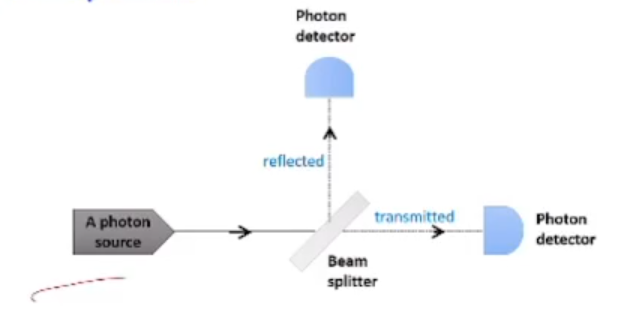
\includegraphics[scale=0.5]{1.png}
\end{center}
We send a series of individual photons along a path from the source towards the splitter. We expect two behaviors: the beam splitter transmits or reflects the photon. We observe the photon arriving at the detector on the right of the splitter half of the time, and arriving at the detector above half of the time.\\
So, we can model the splitter as flipping a fair coin, and choosing whether to transmit or reflect the photon based on the result of the coin-flip.\\\\
A beam splitter behaves like a fair coin: head (state 0) $\rightarrow$ transmitted, tail (state 1) $\rightarrow$ reflected. So both detectors will expect a photon with probability $\frac{1}{2}$
\subparagraph{Second experiment} We extend the experiment with two mirrors and another beam splitter.
\begin{center}
	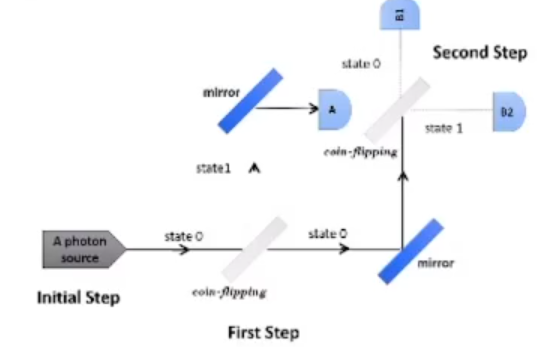
\includegraphics[scale=0.5]{2.png}
\end{center}
We have three detectors, and we observe a photon in A with probability $\frac{1}{2}$, and in B1 or B2 with probability both $\frac{1}{4}$.\\
Both experiments confirms our prediction.
\subparagraph{Third experiment} Let's remove the detector A.\begin{center}
	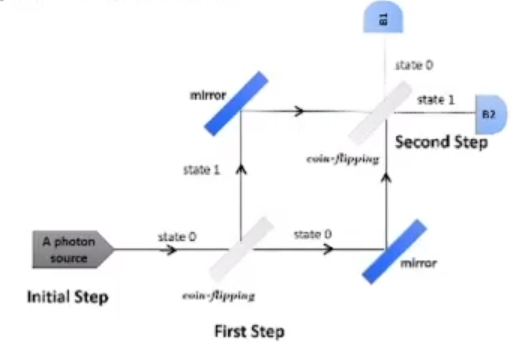
\includegraphics[scale=0.5]{3.png}
\end{center}
So we flip our photon, the "quantum coin", \textbf{without looking at the result of the first splitter}. What are the probabilities of observing the photon in B1 or B2? With the classical intuition, we expect $\frac{1}{2}$ probability in both and that's what would happen with a real "macroscopic" coin. So we predict to observe the photon in B1 and B2 evenly.\\
Let's see it in a mathematical way:
\begin{list}{}{}
	\item State 0: transmitted
	\item State 1: reflected
\end{list}
With a vector representation:
$$|0\rangle = \left(\begin{array}{c}
	1\\0
	\end{array}\right)\:\:\:\:\:\:\:\:|1\rangle = \left(\begin{array}{c}
	0\\1
	\end{array}\right)$$
With $|\:\:\rangle$ called \textbf{Dirac notation}, standard notation for states in quantum mechanics.\\
Uncertain states will be represented by linear combinations of $|0\rangle$ and $|1\rangle$
$$\alpha_0|0\rangle + \alpha_1|1\rangle = \alpha_0\left(\begin{array}{c}
1\\0
\end{array}\right) + \alpha_1\left(\begin{array}{c}
0\\1
\end{array}\right) = \left(\begin{array}{c}
\alpha_0\\\alpha_1
\end{array}\right)$$
With $\alpha_0,\alpha_1$ being the probabilities of finding the photon in state $|0\rangle$ or $|1\rangle$.\\
Since we should find the photon in exactly one path, we must have $\alpha_0+\alpha_1=1$\\\\
We model the splitter as randomly selecting whether the photon will be transmitted (state $|0\rangle$) or reflected (state $|1\rangle$)\\
After the initial step, we are in $|0\rangle$. We flip a coin (first splitter): the new probabilistic state is expected to be in both states with probability $\frac{1}{2}$
$$\frac{1}{2}|0\rangle + \frac{1}{2}|1\rangle = \left(\begin{array}{c}
\frac{1}{2}\\\frac{1}{2}
\end{array}\right)$$
The transition of a far coin can be represented by the matrix $$\left(\begin{array}{c c}
\frac{1}{2}&\frac{1}{2}\\\frac{1}{2}&\frac{1}{2}
\end{array}\right)$$
When the photon passes through the splitter, we multiply its state vector by this matrix, to derive the new state where the photon is expected to be in both states $|0\rangle$ and $|1\rangle$ with probability $\frac{1}{2}$
$$\left(\begin{array}{c c}
\frac{1}{2}&\frac{1}{2}\\\frac{1}{2}&\frac{1}{2}
\end{array}\right)\left(\begin{array}{c}
1\\0
\end{array}\right) = \left(\begin{array}{c}
\frac{1}{2}\\\frac{1}{2}
\end{array}\right) = \frac{1}{2}\left(\begin{array}{c}
1\\0
\end{array}\right) + \frac{1}{2}\left(\begin{array}{c}
0\\1
\end{array}\right)$$
Then we flip the coin again, and multiply the new state vector by the same matrix. The new probabilistic state will be the same:
$$\left(\begin{array}{c c}
\frac{1}{2}&\frac{1}{2}\\\frac{1}{2}&\frac{1}{2}
\end{array}\right)\left(\begin{array}{c}
\frac{1}{2}\\\frac{1}{2}
\end{array}\right) = \left(\begin{array}{c}
\frac{1}{2}\\\frac{1}{2}
\end{array}\right) = \frac{1}{2}\left(\begin{array}{c}
1\\0
\end{array}\right) + \frac{1}{2}\left(\begin{array}{c}
0\\1
\end{array}\right)$$
So our mathematical model confirms our expectations.\\\\
\textbf{The experimental results do not agree with our classical intuition!} We observe the photons \textbf{only in B1} and we \textbf{never observe any photon in B2}. This is the same problem which led to the development of quantum physics.
\paragraph{Quantum Physics} So let's use quantum physics to explain our experiments. "\textit{Quantum theory is probability theory with negative numbers}", but we can't have negative probabilities so we will use a new quantity called \textbf{amplitude}. To get around the fact that we cannot have negative probabilities and that all our probabilities must add up to 1, we use a mathematical trick: we square our amplitudes to calculate the probabilities.\\
According to the quantum mechanical description, the beam splitter causes the photon to go into a \textbf{superposition} of both states. Mathematically, we describe such superposition by taking a linear combination of the state vectors with $\alpha_0$ and $\alpha_1$ now being \textbf{complex numbers} $\in C$. If we measure the photon to see its state, we find it in state $|0\rangle$ with probability $|\alpha_0|^2$ and in state $|1\rangle$ with probability $|\alpha_1|^2$, and since a photon should be find in exactly one path, we need $|\alpha_0|^2+|\alpha_1|^2 = 1$\\\\
We start in state $|0\rangle=\left(\begin{array}{c}1\\0\end{array}\right)$. When it passes through the first splitter, we multiply its state vector with the matrix $$\left(\begin{array}{c c}
\frac{1}{\sqrt{2}}&\frac{1}{\sqrt{2}}\\\frac{1}{\sqrt{2}}&-\frac{1}{\sqrt{2}}
\end{array}\right)$$
After passing through the first splitter:
$$\left(\begin{array}{c c}
\frac{1}{\sqrt{2}}&\frac{1}{\sqrt{2}}\\\frac{1}{\sqrt{2}}&-\frac{1}{\sqrt{2}}
\end{array}\right)\left(\begin{array}{c}
1\\0
\end{array}\right) = \left(\begin{array}{c}
\frac{1}{\sqrt{2}}\\\frac{1}{\sqrt{2}}
\end{array}\right) = \frac{1}{\sqrt{2}}\left(\begin{array}{c}
1\\1
\end{array}\right)$$
Same as before, with $\frac{1}{\sqrt{2}}$ instead of $\frac{1}{2}$. The result correspond with the observed behavior: we measure the photon in state $|0\rangle$ with probability $\left(\frac{1}{\sqrt{2}}\right)^2=\frac{1}{2}$ and in state $|1\rangle$ with probability $\left(\frac{1}{\sqrt{2}}\right)^2=\frac{1}{2}$. The photon is in a \textbf{superposition} of states $|0\rangle$ and state $|1\rangle$, being in both states with amplitudes $\frac{1}{\sqrt{2}}$ and $\frac{1}{\sqrt{2}}$ respectively.\\
If we do not measure the state of the photon after passing through the first beam splitter, then its state remains $\frac{1}{\sqrt{2}}\left(\begin{array}{c}
1\\1
\end{array}\right)$. If the photon is allowed to pass through the second splitter before any measurement, the new state vector becomes
$$\left(\begin{array}{c c}
\frac{1}{\sqrt{2}}&\frac{1}{\sqrt{2}}\\\frac{1}{\sqrt{2}}&-\frac{1}{\sqrt{2}}
\end{array}\right)\cdot\frac{1}{\sqrt{2}}\left(\begin{array}{c}
1\\1
\end{array}\right) = \left(\begin{array}{c}
\frac{1}{2} + \frac{1}{2}\\\frac{1}{2}-\frac{1}{2}
\end{array}\right) = \left(\begin{array}{c}
1\\0
\end{array}\right)$$
The amplitude of the state $|0\rangle$ becomes 1, but the amplitude of the state $|1\rangle$ becomes 0 because \textbf{the amplitudes of finding the photon in state $|1\rangle$ cancel each other out}. We call this effect \textbf{interference}.\\
After being in both states at the same time with certain amplitudes, by passing through a second splitter the outcomes are interfered with each other: the interference can be destructive ($\frac{1}{2} - \frac{1}{2}$) or constructive ($\frac{1}{2} + \frac{1}{2}$).
\paragraph{What is Quantum Computing?} If we measure the photon, we find it coming out of state $|0\rangle$ with probability 1. Thus, after the second splitter the photon is entirely in state $|0\rangle$, which is what we observed.\\
In quantum "language": the second splitter has caused the two states (in superposition) to interfere, resulting in the cancellation of state $|1\rangle$.\\
The interference effects can be used to our advantage. We can combine operations such as the quantum coin toss to build more efficient algorithms. These algorithms can use interference effects to make the wrong answers cancel out quickly and give us high probabilities of measuring the right answer. This is the idea behind quantum computing.
\paragraph{Observations}\begin{list}{}{}
	\item This model works when the initial state is $|1\rangle$
	\item This model works also with complex numbers\\
	For instance we could use:
	\begin{list}{}{}
		\item Transition matrix: $\frac{1}{\sqrt{2}}\left(\begin{array}{c c}
		1&i\\i&1
		\end{array}\right)$
		\item Superposition of state $|0\rangle$ and $|1\rangle$: $\frac{1}{\sqrt{2}}\left(\begin{array}{c}
		i\\1
		\end{array}\right)$
		\item The model is consistent with the first and second experiment
		\begin{center}
			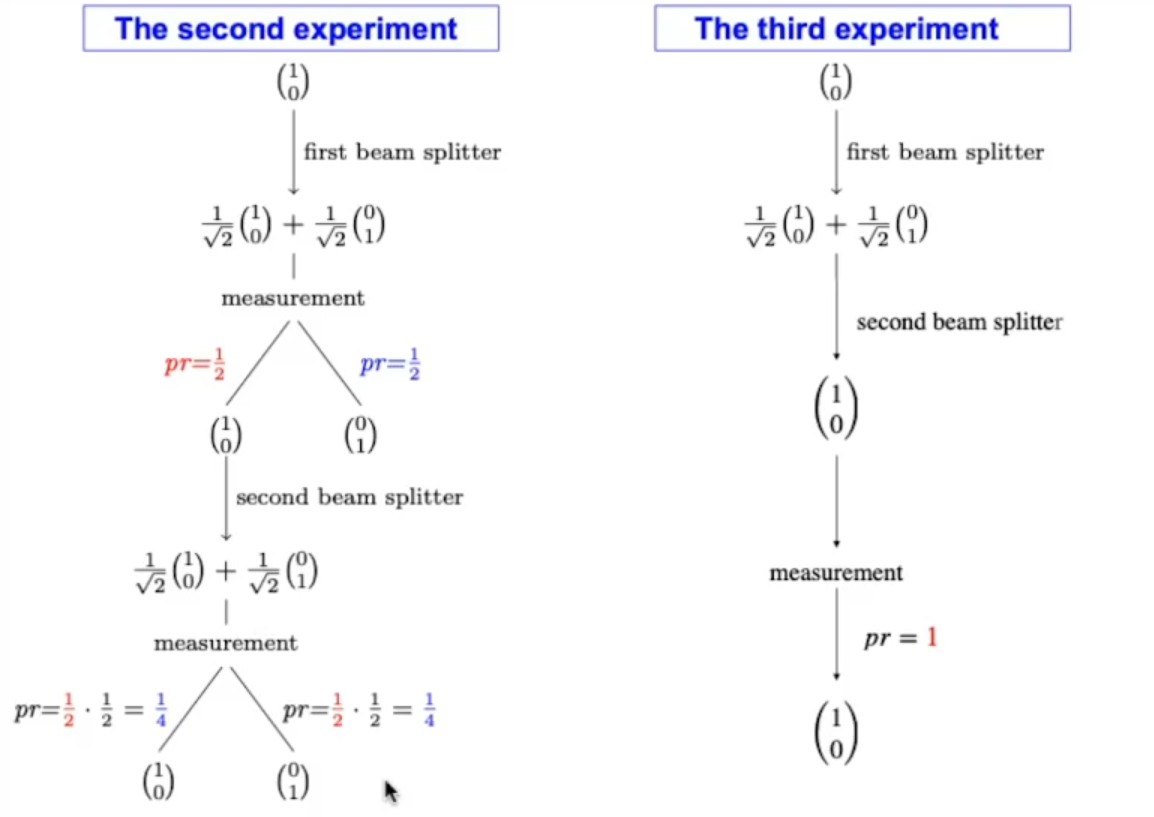
\includegraphics[scale=0.5]{4.png}
		\end{center}
	\end{list}
\end{list}
\paragraph{Phenomena of quantum mechanics that may intervene in the processing of information}
\begin{list}{}{}
	\item \textbf{Superposition} Property of a quantum system to be in different states at the same time.\\
	A quantum system can be in more than one state at the same time with non-zero amplitudes: we say that it's in a superposition of these states. When evolving from a superposition, the resulting transitions may affect each other constructively and destructively. This happens because of having opposite sign transition amplitudes
	\item \textbf{Decoherence} The attempt to observe or measure the state of the system causes its collapse towards a single state.\\
	The probability of a system to be observed in a specific state is the square value of its amplitude of a state. After the measurement, the system is no longer in a superposition: the information kept in the superposition is lost.\\
	The experimental manipulation of quantum systems is extremely difficult because every minimal disturbance can determine the decoherence.\\
	Qubits interact with their environments to some degree, even thought the physical substrate used to store them has been designed to keep the isolated.
	\item \textbf{No-Cloning} It's impossible to create an independent and identical copy of an arbitrary unknown quantum state
	\item \textbf{Entanglement} Possibility that two or more elements are in quantum states completely correlated with each other so that, even if transported at a great distance from each other, they maintain the correlation.
\end{list}
\subsection{Quantum Computer}
\paragraph{Bit and qubit} Conventional computers are made up of bits, while quantum computers are made up of quantum bits, or \textbf{qubits}.\\
A bit is the fundamental concept of classical computation: we can think of it in abstract terms as having a state which is either 0 or 1.\\
A qubit is the simplest of all quantum systems:
\begin{list}{}{}
	\item like a bit, it has a state
	\item two special states for qubits are the state $|0\rangle$ and $|1\rangle$, which correspond to states 0 and 1 of classical bits
	
$$|0\rangle = \left(\begin{array}{c}
	1\\0
	\end{array}\right)\:\:\:\:\:\:\:\:|1\rangle = \left(\begin{array}{c}
	0\\1
	\end{array}\right)$$
	These are called \textbf{computational basis states} and form an orthonormal basis for $C^2$
	\item The difference between bits and qubits is that a qubit can be in a state other than $|0\rangle$ and $|1\rangle$: it can be in a superposition of the two states simultaneously
	$$|\psi\rangle = \alpha|0\rangle+\beta|1\rangle$$
	\item The representation of information is binary, but each qubits contains double information with respect to a bit.
	\item We can examine a bit to determine if it's in state 0 or 1, but we cannot examine a qubit to determine it's quantum state (the values of $\alpha$ and $\beta$). We can only acquire much more restricted information about the quantum state.
	\item Measuring a qubit can only give classical results: either 0 with probability $|\alpha|^2$ or 1 with probability $|\beta|^2$\\
	Note that by measuring we lose information.
	\item A qubit $|\psi\rangle$ can be represented in a three-dimensional space as a point on the surface of a sphere of unitary radius known as \textbf{Bloch's sphere}.
\end{list}
\begin{center}
	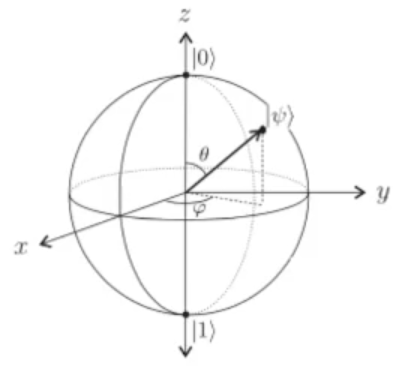
\includegraphics[scale=0.5]{5.png}
\end{center}
How much information in a qubit $|\psi\rangle = \alpha|0\rangle + \beta|1\rangle$? $\alpha$ is a complex number and we could store lots of bits in the binary expression of Re$(\alpha)$. This is there was some way of measuring the value of $\alpha$ exactly. But $\alpha,\beta$ are kind of hidden information. Measurement of a qubit will give only a single bit of information, 0 or 1, about the state of the qubit. There is no way to figure out $\alpha$ and $\beta$ if they start out unknown: after the measurement $\alpha$ and $\beta$ are gone.\\
Why does this collapse occurs? \textbf{We don't know}.\\
Only if infinitely many identically prepared qubits %TODO
\paragraph{Power of Quantum Computing} The system can be put in a combination of very large number of state: $n$ qubits in a superposition of $2^n$ states, so operating on $2^n$ bits at the same time.\\
Idea: find an algorithm that converges all $2^n$ states of the qubits to a state that's solution of the problem: exploiting constructive and destructive interferences, for example.
\paragraph{Quantum Algorithms} We start from a well known initial state (example: all qubits in $|0\rangle$). The system evolves in a quantum way: qubits are connected in elementary logic circuits and are manipulated by a simple set of rules (rotations of state vectors of the quantum state).\\
From a superposition of states to a superpositions of calculations (each with a certain probability of converging to a significant result) to a superposition of results. When the machine measures the final state, the superposition of results collapses on the result with the higher probability: with high probability being the solution of our problem.\\
This can be called \textbf{quantum parallelism}.\begin{list}{}{}
	\item Observing the system during these manipulations comes with a severe \textbf{penalty}: if we look to soon, the \textbf{computation will fail}. We are allowed to \textbf{view only the machine final state}.
	\item Interaction with the outside occurs through classic bit sequences: qubits collapses in that instant to a single state.
\end{list}
\paragraph{Why Quantum Computing?} The idea was born to efficiently simulate quantum-mechanical processes. But this model can help to solve problems of high computational complexity.\\
However:
\begin{list}{}{}
	\item Quantum computation doesn't violate the Church-Turing thesis, undecidable functions are still undecidable
	\item Widely believed that NP-Complete problems are still difficult problems, requiring exponential time
\end{list}
We are interested because for some problems a classical computers can take exponentially more time.
\paragraph{Shor's Factoring Algorithm} Factor numbers in polynomial time. This remains one of the (or \textit{the}) most important results in quantum computing. Meaning that \textbf{current public key cryptography can be attacked}. But remember that factorization is not NP-complete.
\paragraph{Grover's Quantum Search} The algorithm concerns search in an unstructured database with $N$ entries. If we are searching for a unique marked entry, classicaly it would take a maximum of $N$ queries and $\frac{N}{2}$ queries on average.\\
With this algorithm, enables the search to be completed with $O(\sqrt{N})$ queries. It's \textbf{optimal}: no search algorithm can do less than $\sqrt{N}$ operations.\\
In practice, this quadratic speed-up can be very impactful making a big difference. With $10^{20}$ entries, and a quantum processors capable of $10^8$ calls per second, we can find the entry in $10^{10}$ calls, so $10^2$ seconds ($\simeq 2$ minutes). In classical search we would need $10^{12}$ seconds ($\simeq 32000$ years).\\
In cryptography, it enables brute force attacks so we need longer keys.
\paragraph{Evolution of Quantum Technology}
%TODO image
\begin{center}
	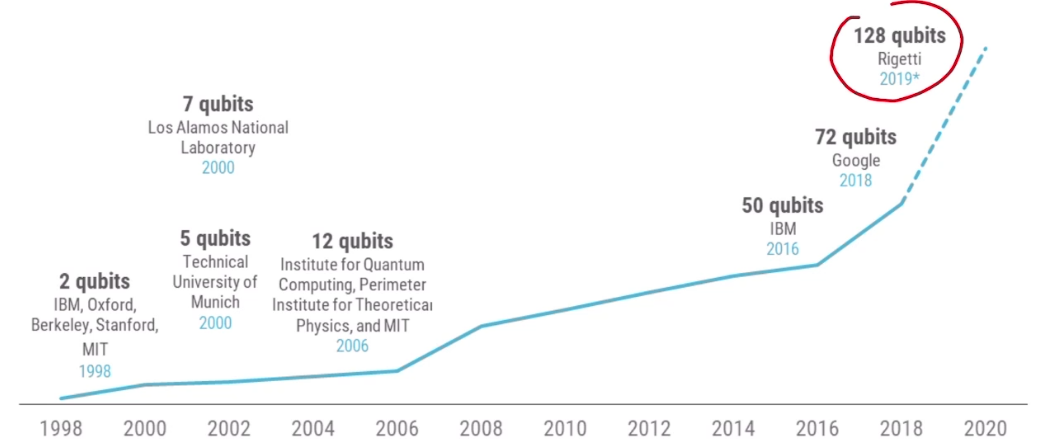
\includegraphics[scale=0.5]{6.png}
\end{center}
IBM claims that it will build a 1000-qubit machine by 2023 and 1M-qubits by 2030.
\paragraph{Quantum Supremacy} Is the goal of demonstrating that a programmable quantum device can solve a problem that \textbf{no classical computer can solve in any feasible amount of time} (irrespective of the usefulness of the problem).\\
Proving this requires:\begin{list}{}{}
	\item Building a powerful physical quantum machine
	\item Finding a problem that can be solved efficiently on a quantum computer with a superpolynomial speed-up over the best known or possible classical algorithm for that task.
\end{list}
Note that Shor's algorithm is unfeasible to be implemented with current technology, so it cannot be used to prove quantum supremacy.
\paragraph{Physical Realization of Quantum Computers}
A qubit can be realized as real quantum physical system. We can use:
\begin{list}{}{}
	\item Two different polarization of a photon
	\item Two possible alignments of nuclear spin in a uniform magnetic field
	\item Two state of an electron orbiting a single atom (ground or excited state, shining light on the electron makes it change states and even stay halfway between states)
\end{list}
The theory is independent of the physical realization of the system.
\begin{center}
	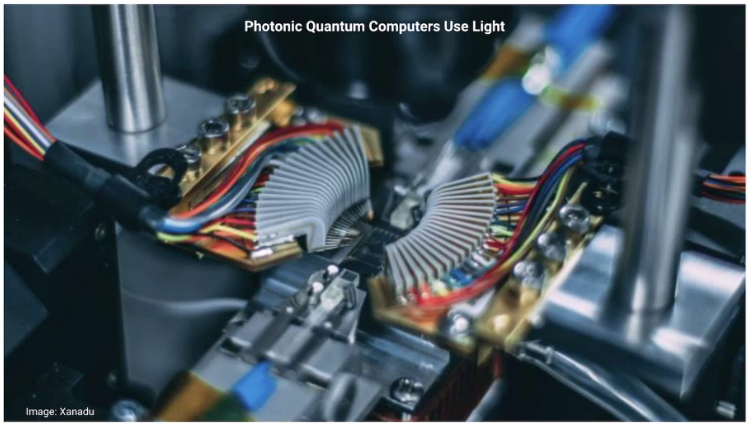
\includegraphics[scale=0.5]{7.png}
	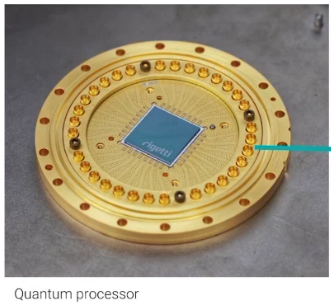
\includegraphics[scale=0.7]{8.png}
\end{center}
\paragraph{Challenges} It will be quite an engineering challenge to control a quantum computer and to make sure that its state will not be affected by various sources of error.\\
Quantum operations (rotations) are never perfect: an intended rotation of 90 degrees might end up being of 90.1 or 89.9 degrees and this errors add up quickly.\\
It's very difficult to avoid interaction with the external environments, so need fault-tollerant protocols and quantum-errors correcting algorithms, meaning additional qubits.\\
Circuit dimensions are also very large. Shor's algorithm require $O(n^2\log n\log\log n)$ gates for a $n$ bit number.
\section{Circuit Model of Computation}
\begin{center}
	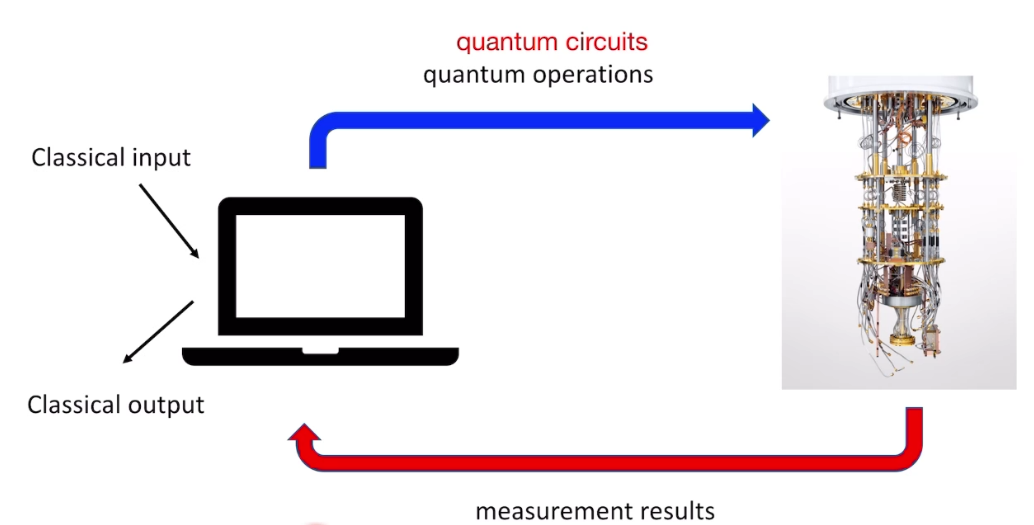
\includegraphics[scale=0.5]{9.png}
\end{center}
The \textbf{interaction is classical}.
\paragraph{Circuits} Networks (graphs) of wires (arcs) that carry bit values to gates that perform elementary operations (nodes) on the bits (input nodes).\\
$C_n$ circuit with $n$ input variables. We consider acyclic circuits. The gates come from some finite library of gates.\\
Circuits are a \textbf{non-uniform model of computation}: with $n$ inputs we can solve only instances of length $n$. Inputs of different lengths are processed by different circuits, in contrast with uniform models (such as Turing machines) where the same computational device is used for all possible input lengths. A different "program" for each input size.\\\\Non-uniform because computation on input size $n$ can be absolutely different from computations on some input size $m$. For example, \textbf{non-uniform circuit families of small size may compute undecidable functions}. Size being the number of operations in the circuit.\begin{list}{}{}
	\item Let $L\subseteq \{0,1\}^*$ be an undecidable language
	\item Let $U = \{1^n\:|\:$the binary expansion of $n$ is in $L\}$\\
	For example $1^5 = 11111_1\in U$ if $5_{10}=101_2 \in L$
	\item $U$ is also undecidable, but we can build a non-uniform family of circuits that computes $U$: $\forall\:n$ we build two circuits with $n$ inputs\begin{list}{}{}
		\item $C_n^0$ that outputs 0 if $1^n\not\in U$
		\item $C_n^1$ that outputs 1 if $1^n\in U$
	\end{list}
	What's missing is the \textbf{effective and efficient constructability} of the circuits. Since $U$ is undecidable we are not able to say if the $n$-th circuit of the family is $C_n^0$ or $C_n^1$.
\end{list}
\paragraph{Uniform Families} So we often impose a \textbf{uniformity condition}: the family is uniform if each $C_n$ can be constructed by an appropriately resource-bounded Turing machine. We assume that the circuits can be generated by a Turing machine or equivalent model that on input $n$ produces a description of $C_n$ in time polynomial in $n$ and in the number of gates in $C_n$.
\paragraph{Complexity of the Circuits} One natural measure is the \textbf{overall number of gates}, the number of operations (can be put in relation with sequential time).\\
Another is the \textbf{depth of the circuit}, the length of the longest path between input and output with each gate counting as one, can be put in relation with parallel time.\\
A third measure is the \textbf{number of input variables}, sometimes called width or space of the circuit.
\paragraph{Reversible Computation} Quantum computation are always reversible. A computation is reversible if it always possible to uniquely recover the input given the output. Otherwise, it's called irreversible.\\
Many classical logic gates are irreversible, but the NOT gate is reversible.\\
Reversibility is connected to information loss: an irreversible operation produces loss of information. With reversible computation no information is ever erased.\\
\textbf{Laws of physics are fundamentally reversible}, per out present understanding: theory of quantum computing is related to a theory of reversible computing \textbf{so quantum circuits must be reversible}.
\paragraph{Reversible Circuits} Realize bijection. We have digital circuits with same number of input and outputs. Any classical irreversible circuit can be transformed in a equivalent reversible one (computes same one), by adding new inputs and new outputs and replacing irreversible operations with reversible ones. The extra inputs represent information that we must keep in order to maintain the reversability.\\
With an irreversible classical circuit of depth $T$ and space $S$, the reversible version uses $O(S+ST)$ space and $T$ depth.
\subparagraph{Reversible AND} Also known as Toffoli gate.
\begin{center}
	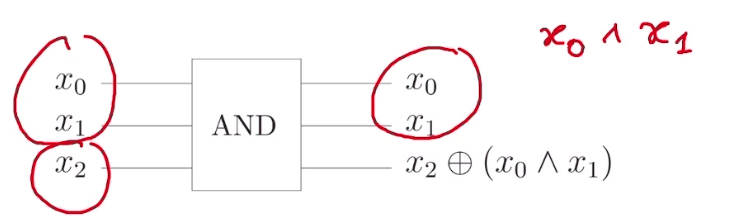
\includegraphics[scale=0.5]{10.png}
\end{center}
\paragraph{Universality} A set of gates is universal for classical computation if, for any positive integer $n,m$ and any function $f : \{0,1\}^n\rightarrow \{0,1\}^m$, a circuit can be constructed for computing $f$ using only gates from that set.\\
Well-known sets are \{AND, OR, NOT\}, \{AND, XOR, NOT\}, \{NAND\}, \{NOR\}:  NAND and NOR gates have the \textbf{functional completeness} property assuming unlimited fanout (a gate can be connected to unlimitedly many nodes).\\\\
\textbf{Toffoli gate} is universal for classical reversible computation. We need to add \textbf{ancillary} (extra) bits that can be initialized to 0 or 1 as required.
\section{Complex Numbers}
A field that can be represented in a 2D space.
$$z = a + ib$$ with $a,b \in R$ and $i^2 = -1$, that can be represented in a plot with $Re(z) = a$ on $x$ axis and $Im(z) = b$ on $y$ axis (\textbf{cartesian form}).\\
Can be expressed also as $$z = \rho(\cos\theta + i \sin\theta) = \rho \cdot e^{i\theta}$$ with $\rho$ being the distance from the origin and $\theta$ the angle (\textbf{polar form}). $\rho$ is called modulo and $e^{i\theta}$ is called phase (sometimes referring with that term to just $\theta$)
$$|z|^2 = z\cdot z^* = a^2 + b^2 = \rho^2 = |z^*|$$
$$z^* = \overline{z} = a-ib = \rho(\cos\theta - i\sin\theta) = \rho\cdot e^{-i\theta}$$
with $\overline{z}$ called complex conjugate of $z$.
\paragraph{Euler Identity} Let's prove the polar form. $e^z$ is a function from $C$ to $C$
$$e^z = \sum_{k=0}^\infty = \frac{z^k}{k!}$$
With $z\in C$, let's see with $z = ix$ and $x\in R$. We want to prove that
$$e^{ix} = \cos x + i\sin x$$
\pagebreak
$$e^{ix} = \sum_{k=0}^\infty \frac{(ix)^k}{k!} = 1 + ix + \frac{i^2x^2}{2} + \frac{i^3x^3}{3!} + \ldots=$$
Let's take the even powers, we have $i^2 = -1, i^4 = +1,\ldots$, and with the odd powers we can take out $i$ from the $\sum$
$$= \sum_{k=0}^\infty \frac{(-1)^{k}x^{2k}}{(2k)!} + i\sum_{k=0}^\infty \frac{(-1)^k x^{2k+1}}{(2k+1)!} =$$
These are the power series expansions of $\cos$ and $\sin$
$$e^{ix}=\cos x + i \sin x$$
This results in the Euler identity which puts together all the principle of math. The imaginary unit an two irrational number together with $1$ and $0$.
$$e^{i\pi} + 1 = 0 \Leftrightarrow e^{i\pi} = -1$$
\paragraph{Roots of Unity} Useful when we want to solve $z^n - 1 = 0$. We know that every polynomial has exactly $n$ roots in $C$\\
Primitive $n$th root of 1
$$\omega_n = e^{\frac{2\pi i}{n}} = \cos \frac{2\pi}{n} + i \sin\frac{2\pi}{n}$$
So for example $\omega_3 = \cos\frac{2}{3}\pi + i\sin\frac{2}{3}\pi = \frac{1}{2}+i\frac{\sqrt{3}}{2}$ for $z^3 - 1 = 0$\\
So they are counterclockwise on the unitary circle and also unitary roots are cyclic
$$w_n^k = (\cos \frac{2\pi}{n} + i \sin\frac{2\pi}{n})^k = \cos\frac{2\pi}{n}k + i \sin\frac{2\pi}{n}k = \left(e^{\frac{2\pi i}{n}}\right)^k$$
\begin{list}{}{}
	\item $\omega_n^0 = 1$
	\item $\omega_n^{n+k} = \omega_n^n \cdot \omega_n^k = \omega_n^k$
	\item $\omega_n^{n-k} = \omega_n^n \cdot \omega_n^{-k} = \omega_n^{-k}$
\end{list}
Multiplication and division are easier in the polar form
$$z_1\cdot z_2 = \rho_1\cdot\rho_2(\cos(\theta_1+\theta_2) + i\sin(\theta_1+\theta_2))$$
$$\frac{z_1}{z_2} = \frac{\rho_1}{\rho_2}(\cos(\theta_1-\theta_2) + i\sin(\theta_1-\theta_2))$$
$$z^n = \rho^n\cdot e^{in\theta}$$
\subsection{Hilbert Spaces} For Quantum Computing only finite dimensional Hilbert spaces meaning complex vector spaces with an inner product.
\paragraph{Definition} A quantum state space of a system is a vector space (complex) with inner product.\\
For example, photon polarization: we have a basis and it's a 2-dimensional space. Base states are $|\updownarrow\rangle$ and $|\leftrightarrow\rangle$. We use half-spin patches, $|\uparrow\rangle$ spin up and $|\downarrow\rangle$ spin down.\\
If we consider a 4-dimensional state space, we have $4$ vectors in the base:$|0\rangle$, $|1\rangle$, $|2\rangle$, $|3\rangle$ denoted with $$|v\rangle=\left(\begin{array}{c}
v_0\\v_1\\v_2\\v_3
\end{array}\right)$$ using the ket notation.
\paragraph{Definition} A quantum state is a vector of unitary length in a quantum state space.\\
So $\| |v\rangle\| = 1$, $\|v\|=\sqrt{(v,v)}$ with the inner product defined as
$$(v,w)=\sum_{i=1}^{d-1}v_i^*\cdot w_i$$
We can use the bra $$\langle v| = (v_0^*,\ldots,v_{d-1}^*)$$
$$\langle v\:|\:w\rangle = (v,w)\in C$$
or the ket-bra $$|v\rangle\langle w| = (v_iw_j^*)_{i,j}$$ giving a rank-one matrix.
\paragraph{} For a system of 1 qubit we have as basis $$|0\rangle = \left(\begin{array}{c}
1\\0
\end{array}\right), |1\rangle=\left(\begin{array}{c}
0\\1
\end{array}\right)$$ but we can also denote this as $|\uparrow\rangle$ and $|\downarrow\rangle$ and denote as $$|\rightarrow\rangle = \frac{|\uparrow\rangle + |\downarrow\rangle}{\sqrt{2}}$$
$$|\leftarrow\rangle = \frac{|\uparrow\rangle - |\downarrow\rangle}{\sqrt{2}}$$
as spin-right and spin-left.\\
We can define spin-in ("in the board")
$$|\otimes\rangle = \frac{|\uparrow\rangle + i|\downarrow\rangle}{\sqrt{2}}$$
and spin-out ("out of the board")
$$|\bullet\rangle = \frac{|\uparrow\rangle - i|\downarrow\rangle}{\sqrt{2}}$$
Multiplying a quantum state bu a global phase ($e^{i\theta}$) we do not change the nature of the quantum state. A global phase is a quantity that multiply all the components of the basis vector.
$$|\rightarrow\rangle = \frac{|\uparrow\rangle + |\downarrow\rangle}{\sqrt{2}} \neq \frac{|\uparrow\rangle + i|\downarrow\rangle}{\sqrt{2}} = |
\otimes\rangle$$
In the above case, $i$ is a relative phase.
\paragraph{Bloch Sphere} %TODO
\begin{center}
	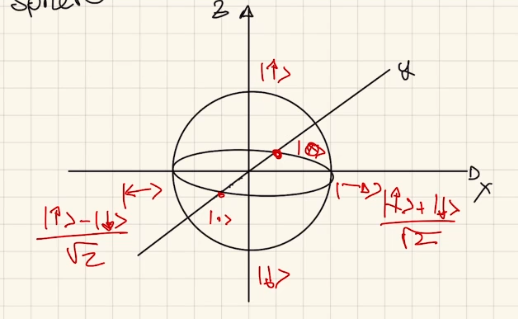
\includegraphics[scale=0.5]{11.png}
\end{center}
\paragraph{Pauli Matrices} $$X = \sigma_x = \left(\begin{array}{c c}
0&1\\1&0
\end{array}\right)$$
$$\sigma_x|0\rangle = \left(\begin{array}{c c}
0&1\\1&0
\end{array}\right)\cdot\left(\begin{array}{c}
1\\0
\end{array}\right) = \left(\begin{array}{c}
0\\1
\end{array}\right) =|1\rangle$$
It reflects the points along the $x$ axis. The same goes for $\sigma_x|1\rangle = |0\rangle$.\\
So for the points on the $x$ axis stay almost the same.
$$|\rightarrow\rangle = \frac{|0\rangle + |1\rangle}{\sqrt{2}} = \frac{1}{\sqrt{2}}\left(\begin{array}{c}
1\\1
\end{array}\right)$$
$$\sigma_x|\rightarrow\rangle = \frac{1}{\sqrt{2}}\left(\begin{array}{c}
1\\1
\end{array}\right)$$
The $y$ axis Pauli matrix is $$Y = \sigma_y = \left(\begin{array}{c c}
0&-i\\i&0
\end{array}\right) = -i|0\rangle\langle1| + i |1\rangle\langle0|$$
and the last is $$Z = \sigma_z = \left(\begin{array}{c c}
1&0\\0&-1
\end{array}\right) = |0\rangle\langle0| - |1\rangle\langle1|$$
\subparagraph{Theorem} The three Pauli matrices anticommutes
$$\sigma_i\sigma_j = -\sigma_j\sigma_i$$
for $i,j\in\{x,y,z\}$ and $i\neq j$\\
Also $\sigma_i^2 = I$
\paragraph{Hadamard Matrix} Another important matrix, used for building entangled states.
$$H=\frac{1}{\sqrt{2}}\left(\begin{array}{c c}
1&1\\1&-1
\end{array}\right)$$
It allow to move from the canonical basis to the right-left basis (also known as +- basis).
$$H|0\rangle = \frac{1}{\sqrt{2}}\left(\begin{array}{c}
1\\1
\end{array}\right) = |\rightarrow\rangle = |+\rangle$$
$$H|1\rangle = \frac{1}{\sqrt{2}}\left(\begin{array}{c}
1\\-1
\end{array}\right) = |\leftarrow\rangle = |-\rangle$$
Also $H^2 = I$, $H^{-1} = H$ so $|0\rangle\mapsto_H |+\rangle$ and $|+\rangle\mapsto_H |0\rangle$ same with $|1\rangle$ and $|-\rangle$, "back and forth".\\
$$H|\otimes\rangle = \frac{1}{\sqrt{2}}\left(\begin{array}{c c}
1&1\\1&-1
\end{array}\right)\left(\begin{array}{c}
\frac{1}{\sqrt{2}}\\\frac{1}{\sqrt{2}}i
\end{array}\right) = |\bullet\rangle$$
\paragraph{Other common single qubit gates} Already mentioned $X,Y,Z,H$\begin{list}{}{}
	\item $I = \left(\begin{array}{c c}
	1&0\\0&1
	\end{array}\right)$
	\item $S = \left(\begin{array}{c c}
	1&0\\0&e^{i\frac{\pi}{2}}
	\end{array}\right)$
	\item $T = \left(\begin{array}{c c}
	1&0\\0&e^{i\frac{\pi}{4}}
	\end{array}\right)$
\end{list}
\paragraph{Applying a Gate to a Superposition}
$$\alpha|0\rangle + \beta|1\rangle \mapsto \sigma_x\left(\begin{array}{c}
\alpha\\\beta
\end{array}\right) = \beta|0\rangle + \alpha|1\rangle$$
$$\alpha|0\rangle + \beta|1\rangle \mapsto \sigma_y\left(\begin{array}{c}
\alpha\\\beta
\end{array}\right) = -\beta i|0\rangle + \alpha i|1\rangle$$
$$\alpha|0\rangle + \beta|1\rangle \mapsto \sigma_z\left(\begin{array}{c}
\alpha\\\beta
\end{array}\right) = \alpha|0\rangle - \beta|1\rangle$$
$$\alpha|0\rangle + \beta|1\rangle \mapsto H\left(\begin{array}{c}
\alpha\\\beta
\end{array}\right) = \alpha\left(\frac{|0\rangle + |1\rangle}{\sqrt{2}}\right) + \beta\left(\frac{|0\rangle - |1\rangle}{\sqrt{2}}\right)$$
$$\alpha|0\rangle + \beta|1\rangle \mapsto S\left(\begin{array}{c}
\alpha\\\beta
\end{array}\right) = \alpha|0\rangle + \beta i|1\rangle$$
$$\alpha|0\rangle + \beta|1\rangle \mapsto T\left(\begin{array}{c}
\alpha\\\beta
\end{array}\right) = \alpha|0\rangle + e^{i\frac{\pi}{4}}\beta|1\rangle$$
To really play with qubits we introduce \textbf{unitary transformations}.
\paragraph{Unitary Transformations} A unitary transformation is a transformation mapping unit-vectors to unit-vectors. We are interested in some properties of these unitary transformation.\\
$d$-dimensional quantum state space, it's a vector space so we have a basis: we label the vectors of the base as $$|0\rangle, |1\rangle,\ldots,|d-1\rangle$$
$$|j\rangle = \left(\begin{array}{c}
0\\\vdots\\0\\1\\0\\\vdots\\0
\end{array}\right)\hbox{ with }1\hbox{ in }j\hbox{th position}$$
The unitary transformation is $U = [c_0,\ldots,c_{d-1}]$ so we have $U|j\rangle = |c_j\rangle$: $c_j$ is an unit-vector, because $U$ is a unitary transformation:
\begin{list}{}{}
	\item[1.] $c_j$ is a unit-vector\\All the columns are unit vectors
	\item[2.] We can decompose $U$ as sum of rank-1 matrices
\end{list}
$$U=\sum_{k=0}^{d-1}|c_k\rangle\langle k| = |c_0\rangle\langle 0| + |c_1\rangle\langle 1| + \ldots$$
The matrix $|c_i\rangle\langle i|$ for example is of all 0s with $c_i$ in the $i$th column. $$U|j\rangle = \sum_{k=0}^{d-1}|c_k\rangle\langle k\:|\:j\rangle = \sum_{k=0}^{d-1} |c_k\rangle\delta_{kj}$$
With $\langle k\:|\:j\rangle$ inner product $\in C$ and $\delta_{kj} = \left\{\begin{array}{l l}
0&k\neq j\\
1&k = j
\end{array}\right.$\\
We can apply $U$ to combinations, for example $$U\left(\frac{|k\rangle + |j\rangle}{\sqrt{2}}\right) = \frac{1}{\sqrt{2}}(|c_k\rangle + |c_j\rangle)$$
$$\frac{1}{2}(\langle c_k|+\langle c_j|)(|c_k\rangle + |c_j\rangle) = \frac{1}{2}\left(\langle c_k\:|\:c_k\rangle + \langle c_j\:|\:c_k\rangle + \langle c_k\:|\:c_j\rangle + \langle c_j\:|\:c_j\right)=1$$
$\langle c_j\:|\:c_k\rangle + \langle c_k\:|\:c_j\rangle \in R$ meaning that $\langle c_j\:|\:c_k\rangle$ is pure immaginary, $\in C\setminus R$\\\\
We can also do with relative phases, for example $i|j\rangle$ $$U\left(\frac{|k\rangle + i|j\rangle}{\sqrt{2}}\right) = \frac{1}{\sqrt{2}}\left(|c_k\rangle + i|c_j\rangle\right) = \ldots$$
Ending up with the fact that $\langle c_j\:|\:c_k\rangle$ must be $\in R$.\\
But we have the same quantity pure immaginary and pure real, meaning that $\langle c_j\:|\:c_k\rangle = 0$
\begin{list}{}{}
	\item[3.] Columns of $U$ are orthogonal and also orthonormal
	\item[4.] Rows of $U$ are orthonormal ($\Rightarrow$ orthogonal)
	\item[5.] $U^{-1} = U^H$ \textbf{very important}
\end{list}
$$(U^H)_{ij} = u^*_{ji}$$
And $U^H = U^* =U ^+$, $U^H$ is the conjugate transpose. Diagonal conjugate, invert triangles and transpose elements. An example with an arbitrary, non unitary, matrix:
$$A=\left[\begin{array}{c c}
1+i&2-i\\3+2i&4
\end{array}\right]\Leftrightarrow A^H=\left[\begin{array}{c c}
1-i & 3-2i\\2+i&4
\end{array}\right]$$
\paragraph{Spectral Theorem} There are classes of matrices which have an orthonormal basis of eigenvectors, i.e. are diagonalizable by means of orthogonal matrices.\\
$A = A^T$ symmetric matrices. $\exists$ a orthogonal such that $A = QDQ^T$ with $D$ diagonal matrix with the eigenvalues $\lambda_i$ on the diagonal.\\
$A = A^H$ hermitan matrices, $AA^H = A^HA$\\
\textbf{Unitary matrices are normal matrices}.\\
\textbf{Spectral theorem}: a matrix $A$ is normal $\Leftrightarrow$ $\exists\:U$ unitary and $D$ diagonal $|\:A=UDU^H$, meaning that $Au_i = \lambda_iu_i\:\forall\:i=1,\ldots,n$, i.e. the columns of $U$ are an orthonormal basis of eigenvectors and $\lambda_i$ are the corresponding eigenvalues.
$$A \in C^{n\times n} = UDU^H = \sum_{k=1}^n\lambda_k|u_k\rangle\langle u_k| $$
$$U = [u_1\:|\:\ldots\:|\:u_n]$$
$|u_k\rangle\langle u_k|$ is an example of a \textbf{orthogonal projector} onto the eigenspace corresponding to $\lambda_k$
\paragraph{Evaluation of  systems}
\begin{enumerate}
	\item Isolated processes have a unitary evolution\\
	$|\psi_0\rangle\mapsto|\psi_1\rangle = U_0|\psi_0\rangle\mapsto\ldots$
	\item From time to time the process is "observed", for example with an experiment: this is called \textbf{measurement}.
\end{enumerate}
\paragraph{Rotations} Of an arbitrary angle $\Theta$ around an axis. Three different rotations, for three different axis.\\
A rotation is a unitary matrix that can always be expressed $R_x = e^{-i\frac{\Theta}{2}}x$ (example for axis $x$, same for $z$ and $y$)\\
If $A$ is normal then $A = UDU^H$, so the \textbf{exponential of a matrix} $$e^A = U\left(\sum_{k=1}^\infty \frac{D^{k}}{k!}\right) U^H = Ue^DU^H$$
For example, and since $z$ is diagonal $$R_z(\Theta) = e^{-i\frac{\Theta}{2}z} = \left(\begin{array}{c c}
e^{-i\frac{\Theta}{2}} & 0\\
0 & e^{i\frac{\Theta}{2}}
\end{array}\right) = e^{-i\frac{\Theta}{2}}\left(\begin{array}{c c}
1 & 0\\
0 & -e^{i\Theta}
\end{array}\right)$$
We get that $R_x(\Theta)=(\cos\frac{\Theta}{2})I - i\sin\frac{\Theta}{2}X$, and in general $$R_M(\Theta)=\left(\cos\frac{\Theta}{2}\right)I - i\sin\frac{\Theta}{2}M$$
To diagonalize the matrix $\sigma_i$
$$U\sigma_i U^H = D \Rightarrow e^{-i\frac{\Theta}{2}D}$$
$$U^He^{-i\frac{\Theta}{2}D}U = e^{-i\frac{\Theta}{2}\sigma_i}$$
\paragraph{Theorem} Suppose $U$ is a 1-qubit unitary gate, then there exists real numbers $\alpha,\beta,\gamma,\delta$ such that you can write $U$ like $$U=e^{i\alpha}R_z(\beta)R_y(\gamma)R_z(\delta)$$
$$\Updownarrow$$
$$U = e^{i\alpha}\left[\begin{array}{c c}
e^{-i\frac{\beta}{2}}&0\\0&e^{i\frac{\beta}{2}}
\end{array}\right]\left[\begin{array}{c c}
\cos\frac{\gamma}{2}&-\sin\frac{\gamma}{2}\\\sin\frac{\gamma}{2}&\cos\frac{\gamma}{2}
\end{array}\right]\left[\begin{array}{c c}
e^{-i\frac{\delta}{2}}&0\\0&e^{i\frac{\delta}{2}}
\end{array}\right]$$
Two rotations around $z$ and one around $y$. Any unitary can be decomposed as a product of three rotations times a phase factor.
\paragraph{Standard Rotations}
The standard rotation gates are those that define rotations around the Pauli matrices $X, Y, Z$ and are defined as $$R_P(\theta) = e^{-i\theta\frac{P}{2}} = \cos\left(\frac{\theta}{2}\right)I-i\sin\left(\frac{\theta}{2}\right)P$$
For the $x$ axis
$$R_x(\theta) = \left(\begin{array}{c c}
\cos\left(\frac{\theta}{2}\right)&-i\sin\left(\frac{\theta}{2}\right)\\
i\sin\left(\frac{\theta}{2}\right)&\cos\left(\frac{\theta}{2}\right)
\end{array}\right)$$
For the $y$ axis
$$R_y(\theta) = \left(\begin{array}{c c}
\cos\left(\frac{\theta}{2}\right)&-\sin\left(\frac{\theta}{2}\right)\\
\sin\left(\frac{\theta}{2}\right)&\cos\left(\frac{\theta}{2}\right)
\end{array}\right)$$
For the $z$ axis
$$R_z(\theta) = \left(\begin{array}{c c}
e^{-i\theta\frac{P}{2}}&0\\
0&e^{i\theta\frac{P}{2}}
\end{array}\right)$$
\paragraph{Tensor Products} Way of putting vectors together to form larger Hilbert/vector spaces.\\
Let's assume 2 qubits. The state space of these 2 qubits?
$$|00\rangle\:\:|01\rangle\:\:|10\rangle\:\:|11\rangle$$
The state space dimension is $4$. Which is the dimension of $n$ qubits? Gives us a state space $2^n$.\\
$|01\rangle_{AB} = |0\rangle_A|1\rangle_B = |0\rangle_A\otimes|1\rangle_B$ tensor product.
$$\left(\begin{array}{c}
x\\y
\end{array}\right)\otimes\left(\begin{array}{c}
z\\w
\end{array}\right) = \left(\begin{array}{c}
xz\\xw\\yz\\yw
\end{array}\right)$$
With more dimensions
$$A\otimes B = \left[\begin{array}{c c c}
a_{11}B & \ldots & a_{1n}B\\
\vdots & & \vdots\\
a_{m1}B & \ldots & a_{mn}B
\end{array}\right]$$
For example, $|01\rangle$ encodes 1, meaning "1" in position 1 (counting from 0, so second position)
$$|01\rangle = \left(\begin{array}{c}
1\\0
\end{array}\right)\otimes\left(\begin{array}{c}
0\\1
\end{array}\right) = \left(\begin{array}{c}
0\\1\\0\\0
\end{array}\right)$$

$$|11\rangle = \left(\begin{array}{c}
0\\0\\0\\1
\end{array}\right)$$
$$I\otimes\sigma_x = \left[\begin{array}{c c}
1&0\\0&1
\end{array}\right]\otimes\left[\begin{array}{c c}
0&1\\1&0
\end{array}\right] = \left[\begin{array}{c c c c}
0&1&0&0\\
1&0&0&0\\
0&0&0&1\\
0&0&1&0
\end{array}\right]$$
$$\sigma_x\otimes I = \left[\begin{array}{c c}
0&1\\1&0
\end{array}\right]\otimes\left[\begin{array}{c c}
1&0\\0&1
\end{array}\right] = \left[\begin{array}{c c c c}
0&0&1&0\\
0&0&0&1\\
1&0&0&0\\
0&1&0&0
\end{array}\right]$$
\subparagraph{Degrees of freedom} With 1 qubit $\alpha|0\rangle+\beta|1\rangle$ normalized so the constraint $|\alpha|^2+|\beta|^2 = 1$ and another constraint: we consider the surface of the Bloch sphere of size $2$, so $4-2 = 2$ degrees of freedom.\\
With 2 qubits, $2\cdot4-2$\\
With $n$ qubits $2\cdot 2^n - 2 = 2^{n+1}-2$ degrees\\\\
This argument allows us to say that there must be 2-qubit states that cannot be expressed as product of 2 qubits, because the dimensions do not fit.
$$(\alpha|0\rangle_A+\beta|1\rangle_A)\otimes(\delta|0\rangle_B+\gamma|1\rangle_B)$$
You don't get all the possible configurations of 2-qubits. If $|\psi\rangle = |\psi_1\rangle\otimes|\psi_2\rangle$ so the number of qubits in $\psi$ is equal to the sum of the number of qubits in $\psi_1,\psi_2$, then the system is in a \textbf{separable state}, otherwise the state is \textbf{entangled}.\\
An example of entangled state is the Bell state (EPR state, Einstein Poddsky, Rosen) $$\frac{|01\rangle + |10\rangle}{\sqrt{2}}$$
So no configuration of $\alpha,\beta,\delta,\gamma$ in the previous formula will give the Bell state.
\subparagraph{Inner product of tensor products} Given
$$|\psi\rangle = |\psi_1\rangle\otimes|\psi_2\rangle$$
$$|\phi\rangle = |\phi_1\rangle\otimes|\phi_2\rangle$$
we have that the inner product is
$$\langle \psi\:|\:\phi\rangle = \sum_{i=0}^{d-1}\psi_i\cdot\phi_i = \langle \psi_1\:|\:\phi_1\rangle\langle \psi_2\:|\:\phi_2\rangle$$
Other properties are\begin{list}{}{}
	\item $c(|\psi_1\rangle_A\otimes|\psi_2\rangle) = c|\psi_1\rangle_A\otimes |\psi_2\rangle_B = |\psi_1\rangle_A\otimes c|\psi_2\rangle_B$
	\item $(|\psi_1\rangle_A+|\psi_2\rangle_A)\otimes|\psi_3\rangle_B = |\psi_1\rangle\otimes|\psi_3\rangle_B + |\psi_2\rangle_A\otimes|\psi_3\rangle_B$
	\item $(A\otimes B)(|\psi\rangle_A\otimes|\phi\rangle_B) = A|\psi\rangle \otimes B|\phi\rangle$
	\item $(|\psi\rangle\otimes|\phi\rangle)^* = \langle\psi|\otimes\langle\phi|$
	\item $(A\otimes B)^H = A^H\otimes B^H$
\end{list}
\paragraph{No Cloning Theorem} We cannot make a copy of an \textbf{unknown} qubit.
\subparagraph{Proof} $|\psi\rangle$ unknown qubit in a space of dimension 2, hence $|\psi\rangle|\psi\rangle$ is a space of dimension 4.\\
$|\psi\rangle|0\rangle$ assumes there exists a $U\:|\:U(|\psi\rangle|0\rangle)=|\psi\rangle|\psi\rangle e^{i\theta}$\\
$|\phi\rangle|0\rangle$ assumes there exists a $U\:|\:U(|\phi\rangle|0\rangle)=|\phi\rangle|\phi\rangle e^{i\alpha}$
$$(1\langle\psi|\:_2\langle 0|)U^HU(|\phi\rangle_1|0\rangle_2) = _1\langle\psi|\phi\rangle_1\:_2\langle0|0\rangle_2 = \langle\psi|\phi\rangle$$
Because $\langle0|0\rangle = 1$.\\
We have $U|\phi\rangle_1|0\rangle = |\phi\rangle|\phi\rangle e^{i\alpha}$ and also $\langle\psi|\langle 0|U^H = (U|\psi\rangle|0\rangle)^H = (|\psi\rangle|\psi\rangle e^{i\theta})$
$$(\langle\psi|\langle\psi|)e^{i(\theta-\alpha)}(|\phi\rangle|\phi\rangle) = \langle\psi|\phi\rangle\langle\psi|\phi\rangle = (\langle\psi|\phi\rangle)^2$$
But $\langle\psi|\phi\rangle = (\langle\psi|\phi\rangle)^2 \Leftrightarrow \langle\psi|\phi\rangle = 0 \vee \langle\psi|\phi\rangle = 1$\\
Meaning respectively $|\psi\rangle = |\phi\rangle$ (\textbf{equal states}) $\vee$ $|\psi\rangle$ \textbf{orthogonal to} $|\phi\rangle$
%TODO resto 11/03
\section{Quantum Mechanics}
QM it's \textbf{not a physical theory}, but a \textbf{mathematical theory} composed of four postulates describing the behavior of physical systems. We can think of it as an operating system for the universe, users need another layer (physical theories).
\subsection{Four Postulates}
\paragraph{Closed System} A closed/isolated system is an ideal phyisical system that doesn't interact at all with its environment.
\begin{enumerate}
	\item \textbf{Statics}: describes the state of a closed system
	\item \textbf{Dynamics}: describes the evolution of a closed system
	\item \textbf{Measurement}: describes how information is extracted from a closed system via interactions with an external system
	\item \textbf{Composite Systems}: describes the state of a composite system in terms of its component parts.
\end{enumerate}
\subsubsection{Space-State Postulate} Associated to any physical system there is a \textbf{complex Hilbert space known as the state space of the system}. If the system is isolated, then the system is completely described by its state vector, which is a unit vector in the its state space.
\paragraph{Notes} Tells us that every physical system has a states space, but doesn't tell what the state space is: case-by-case analysis, different physical systems have different state spaces.\\
Always assuming that the state space is described by a vector in a finite-dimensional complex vector space
\paragraph{Qubit} Simplest of all isolated quantum systems, which state space is a two-dimensional complex vector space $C^2$ and its state is described by a unit vector $\in C^2$\\
Any physical system whose state space can be described in $C^2$ can be used to implement a qubit: electrons' spin, photons' polarization\ldots\\
We've seen $|0\rangle$ and $|1\rangle$, the computational basis states which correspond to $0,1$ of the classical bits.\\
We also have the \textbf{normalization constraints} $$\langle\psi\:|\:\psi\rangle = |\alpha|^2+|\beta|^2 = 1$$
And we know that we can describe a qubit in two modes: \textbf{phase factors}. The global phase factor have no physical significance. Relative phase factors between two orthogonal states in superposition are physically significant: two states that differ for a relative phase factor are physically different and not equivalent.\\
Qubits can be geometrically represented as a point on the surface of a sphere of unitary radius called \textbf{Bloch's Sphere}: geometrical representation of a qubit in 3D space. It's limited in representing a single qubit.
\begin{center}
	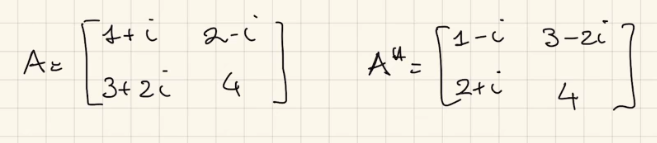
\includegraphics[scale=0.75]{13.png}
\end{center}
%TODO proof of biunivocal representation on the Bloch's sphere.
\begin{list}{}{}
	\item $\theta$ is equivalent to the geometrical latitude: angle with the $z$ axis
	\item $\phi$ is equivalent to the geometrical longitude: angle with the projection on the $(x,y)$ plane and the $x$ axis
\end{list}
\subsubsection{Evolution Postulate}
The time evolution of a closed quantum system is described by the \textbf{Schrodinger Equation} $$ih\frac{d\:|\psi(t)\rangle}{dt} = H(t)\:|\psi(t)\rangle$$
With $h$ being the \textbf{Planck's Constant} and $H(t)$ being the \textbf{fixed Hermitian operator} known as the Hamiltonian of the system.
\paragraph{Notes} The postulate describes the evolution of a quantum system in continuous time, with the change described by a differential equation. The Hamiltonian $H(t)$ represent the \textbf{total energy} function for the system and tells the quantum state how to change.\\
If we know the Hamiltonian of a system, then we understand its dynamics completely (at least in principle). In general, figuring it out is very difficult.
\paragraph{Simplified: Discrete Time Evolution} The discrete time evolution of a closed quantum system is described by a \textbf{unitary transformation}. The state $|\psi\rangle$ of the system at time $t_1$ is related to the state $|\psi'\rangle$ at a later time $t_2$ by a unitary matrix $U$ which depends only on the times $t_1$ and $t_2$ $$|\psi'\rangle = U|\psi\rangle$$
This means applying gates one at the time.
\paragraph{Notes} This expression follows directly form the Schrodinger Equation: every unitary operator $U$ can be realized as a solution of Schrodinger Equation. This postulate, though, doesn't tell us which unitary transformations to use to describe real-world quantum dynamics: case-by-case analysis to figure it out.\\
Unitary matrices because they preserve length.
\paragraph{Measurements} We postulate that closed quantum systems evolve according to a unitary operator. We will be interested in observing and \textbf{measuring} some properties of a system: at some point we must allow the system to interact with the measurement apparatus, making the system no longer closed and the Evolution Postulate no longer appropriate.\\
The evolution of the state of a system during a measurement is not unitary: the third postulate provides a means for describing the effects of measurements on quantum systems.\\
Quantum Systems do get perturbed and modified, and only the probability of observing specific values can be calculated: measurement is a non-deterministic process.
\subsubsection{Measurement Postulate}
Quantum measurements are described by a collection $\{M_m\}$ of measurements operators that satisfy the \textbf{completeness relation} $$\sum_m M_m^+ M_m = I$$
$m$ labels the measurement outcomes that may occur in the experiment. If the state of the quantum system is $|\psi\rangle$ immediately before the measurement, then for each $m$:
\begin{list}{}{}
	\item The probability that result $m$ occurs is given by $$p(m) = \langle\psi|M_m^+M_m|\psi\rangle = \|M_m\:|\psi\rangle\|^2$$
	\item The state of the system after the measurement with outcome $m$ is $$\frac{M_m\:|\psi\rangle}{\sqrt{\langle\psi|M_m^+M_m|\psi\rangle}}$$
\end{list}
\paragraph{Notes} This is only a mathematical formalism for measurements. The state of the system after the measurement is a properly normalized quantum state, and in general it is not a scalar multiple of $|\psi\rangle$: the measurement has modified the state of the system.\\
The denominator vanishes only if $p(m) = 0$, meaning that the result $m$ will never occur.\\
The completeness equation expresses the fact that probabilities sum to one: $$\sum_m p(m) = \sum_m \langle\psi|M_m^+M_m|\psi\rangle = \langle\psi|I|\psi\rangle = \langle\psi|\psi\rangle = 1$$
\paragraph{Example} %TODO
\paragraph{Projective Measurements} For many applications of quantum computation and quantum information we will mostly perform \textbf{projective measurements}, as subset of the possible measurements.\\
Defined in terms of the Hermitian operator: an operator $M$ is Hermitian if it's self-adjoint: $M^+ = M$\\
In physics, Hermitian operators are called observable: \textbf{an observable is a property of a physical system that can be measured} (position, polarization\ldots), and to each physical observable there corresponds an Hermitian operator.\\
All eigenvalues of an observable (so of an Hermitian operator) are real, and the eigenvectors are orthogonal. The \textbf{possible outcomes of a measurement correspond to the eigenvalues of the observable} $M$.\\
Observables can be thought of as questions we can pose to quantum systems: each question admits a set of answers, the eigenvalues of the observable.\\\\Any observable $M$ can be written as its \textbf{spectral decomposition} $$M = \sum_m P_m = \sum_m m|u_m\rangle\langle u_m|$$
\begin{list}{}{}
	\item $m$ are the real eigenvalues of $M$ (outcomes)
	\item $|u_m\rangle$ is the eigenvector associated to $m$
	\item $P_m = |u_m\rangle\langle u_m|$ is the \textbf{projector} onto the eigenspace of $M$ with real eigenvalue $m$
\end{list}
Projectors are operators $P$ which satisfy $P^2 = P$\\
An example is the operator $|0\rangle\langle0|$ $$(|0\rangle\langle0|)^2 = |0\rangle\langle0||0\rangle\langle0| = |0\rangle\:(\langle0|0\rangle)\:\langle0| = |0\rangle\langle0|$$ since $\langle0|0\rangle = 1$
\paragraph{Example} %TODO
\paragraph{Expectation}
$$E_\psi[M] = \langle\psi|M|\psi\rangle$$
\paragraph{Recap on Measurement Postulate} It's a mathematical formalism for measurements. It doesn't tell us what measurement can be done in practice or with what efficiency. Some measurements can be simple to state mathematically but \textbf{not easy to implement}.\\
Tells us how to compute the probability $P(m)$ that outcome $m$ occurs and the new state of the system after the measurement with outcome $m$ applying the measurement operators $M_m$ (one operator for each possible outcome).\\
For projective measurement, these operators, can be derived from the spectral decomposition of the observable $M$ corresponding to the measurement.\\
An observable is a property of a physical system (a \textbf{physical quantity}) that can be measured: position, polarization\ldots Each physical observable corresponds to a \textbf{Hermitian operator}, all eigenvalues of an observable are real and the eigenvectors are orthogonal. The \textbf{possible outcomes of a measurements are the real eigenvalues of $M$}.
Any observable $M$ can be written it as its \textbf{spectral decomposition} $$M = \sum_m mP_m = \sum_m m|u_m\rangle\langle u_m|$$
where \begin{list}{}{}
	\item $m$ are the real eigenvalues, the outcomes of the measurements
	\item $|u_m\rangle$ is the eigenvector associated to $m$
	\item $P_m = |u_m\rangle\langle u_m|$ is the \textbf{projector} onto the eigenspace of $M$ with real eigenvalue $m$
\end{list}
The measurement operators are the projectors $P_m = |u_m\rangle\langle u_m|$\\
The probability of getting result $m$ on the state $|\psi\rangle$ is $$p(m) = \langle\psi\:|\:P_m^+ P_m\:|\:\psi\rangle = \langle\psi|P_m|\psi\rangle $$
Given that outcome $m$ occurred, the state of the quantum system immediately after is $$\frac{P_m|\psi\rangle}{\sqrt{p(m)}}$$
The operators $P_m$ satisfy the completeness relation.
$$\sum_m P_m^+P_m = \sum_m P_m = I$$
\paragraph{Measurements in the Standard Basis} A measurement in the $|0\rangle, |1\rangle$ basis corresponds to perform a projective measurement with projectors $$P_0 = |0\rangle\langle 0| = \left(\begin{array}{c}1//0\end{array}\right) (1\:\:0) = \left(\begin{array}{c c}1&0\\0&0\end{array}\right)$$
$$P_1 = |1\rangle\langle 1| = \left(\begin{array}{c}1//0\end{array}\right) (1\:\:0) = \left(\begin{array}{c c}0&0\\0&1\end{array}\right)$$
Can be seen as projective measurement with respect to Hermitian matrix $Z$
$$Z = |0\rangle\langle 0| - |1\rangle\langle 1| = \left(\begin{array}{c c}
1&0\\0&-1
\end{array}\right)$$
Or also with respect to $I$ with eigenvalues equal to 1
$$I = |0\rangle\langle 0| + |1\rangle\langle 1| = \left(\begin{array}{c c}
1&0\\0&1
\end{array}\right)$$
\paragraph{Measurements in Orthonormal Basis} A measurement in an orthonormal basis $\{|m\rangle\}$ corresponds to perform a projective measurement with projector operators $$P_m=|m\rangle\langle m|$$
For example in the hadamard basis $|+\rangle, |-\rangle$
$$|+\rangle = H|0\rangle = \frac{|0\rangle+|1\rangle}{\sqrt{2}}$$
$$|-\rangle = H|1\rangle = \frac{|0\rangle-|1\rangle}{\sqrt{2}}$$
Corresponds to perform projective measurement with projectors
$$P_+ = |+\rangle\langle +| = \frac{1}{2}\left(\begin{array}{c}
1\\1
\end{array}\right) (1\:1) = \frac{1}{2}\left(\begin{array}{c c}
1&1\\1&1
\end{array}\right)$$
$$P_- = |-\rangle\langle -| = \frac{1}{2}\left(\begin{array}{c}
1\\-1
\end{array}\right) (1\:-1) = \frac{1}{2}\left(\begin{array}{c c}
1&-1\\-1&1
\end{array}\right)$$
And the completeness equation is satisfied $$P_+^+P_+ + P_-^+P_+ = P_+ + P_- = I$$
Single qubit measurements: measuring the identity but also measures the projection over the $x$ axis. All Pauli matrices have eigenvalues of +1 and -1:
$$X = |+\rangle\langle +| - |-\rangle\langle -| = \left(\begin{array}{c c}
0&1\\1&0
\end{array}\right)$$
\subparagraph{Measuring example} Measuring the state $$|\psi\rangle =\alpha|0\rangle + \beta|1\rangle$$
in the $|+\rangle,|-\rangle$ basis gives the result $+$ with probability $$P(+) = \langle\psi|P_+|\psi\rangle = \langle\psi|+\rangle\langle+|\psi\rangle = \frac{1}{2}|\alpha + \beta|^2$$ %TODO
and state after the measurement is $|+\rangle$, while it gives the result $-$ with probability $$P(-) = \langle\psi|P_-|\psi\rangle = \langle\psi|-\rangle\langle-|\psi\rangle = \frac{1}{2}|\alpha - \beta|^2$$ %TODO
and state after is $|-\rangle$.\\
Also relative phase factors are important. Consider the state $|+\rangle,|-\rangle$ differing just for a relative phase factor (plus and minus)
$$|+\rangle = \frac{1}{\sqrt{2}}(|0\rangle + |1\rangle)\:\:\:\:\:|-\rangle = \frac{1}{\sqrt{2}}(|0\rangle - |1\rangle)$$
We cannot distinguish between them by measuring in the computational basis: both 0,1 outcomes occur with probability $\frac{1}{2}$.\\
Considering the $|+\rangle,|-\rangle$ basis, which has measurements operators $P_+,P_-$ if we measure the state $|+\rangle$ we always get outcome $+$, $P(+) = 1, P(-) = 0$. Opposite for measuring $|-\rangle$ getting always $-$ as outcome. So measuring in the $|+\rangle,|-\rangle$ basis distinguish the two state perfectly, relative phase matters.\\
How to measure in a basis different from the computational basis? In the computational basis we have a register, quantum information becomes classical information. How to measure in different basis, for instance the hadamard basis?\\
First we apply a change of basis from the hadamard back to the computational. Then measure respect to the computational and after we change back to the original basis. Example %TODO
We measure either $|0\rangle$ or $|1\rangle$, how to change back? Just apply again the change of basis transformation, since the circuits are always reversible.\\
In general, to implement a measurement with respect to an orthonormal basis $\{\phi_j\rangle\}$:\begin{list}{}{}
	\item The matrix $U$ is applied to perform a basis change to the computational basis
	$$U\left(\sum_j\alpha_j|\phi_j\rangle\right) = \sum_j\alpha_jU|\phi_j\rangle = \sum_j\alpha_j|j\rangle$$
	\item Then a measurement is made in the computational basis obtaining a specific (classical) outcome with probability $|\alpha_j|^2$.\\
	The state of the system after this measurement is $|j\rangle$
	\item Finally $U^{-1}$ is applied to change back to the $\{|\phi_j\rangle\}$ basis, leaving the post-measurement state $|\phi_j\rangle$
\end{list}
\subsubsection{Composition of Systems}
The \textbf{state space of a composite physical system is the tensor product of the state spaces of the component subsystems}. Moreover, if we have systems numbered 1 through $n$, and system number $i$ is prepared in the state $|\psi_i\rangle$, then the joint state of the total system is
$$|\psi_1\rangle\otimes\ldots\otimes|\psi_n\rangle$$
Often $\otimes$ is omitted and the above formula is rewritten as $|\psi_1,\ldots,\psi_n\rangle$\\
Tensor product is the mathematical structure used to describe the state space of a composite physical system because we need a new space which captures the interaction of all $n$ systems.\\
Not all states of acombined system can be separated into the tensor product of states of the individual components.\\
Notation:
\begin{list}{}{}
	\item $|\psi\rangle = \alpha|0\rangle+\beta|1\rangle = \left(\begin{array}{c}
	\alpha\\\beta
	\end{array}\right)$
	\item $|\phi\rangle = \gamma|0\rangle+\delta|1\rangle = \left(\begin{array}{c}
	\gamma\\\delta
	\end{array}\right)$
	\item \textbf{Joint state of the two qubits}
	$$|\psi\rangle\otimes|\phi\rangle = \left(\begin{array}{c}
	\alpha\\\beta
	\end{array}\right)\otimes\left(\begin{array}{c}
	\gamma\\\delta
	\end{array}\right) = \left(\begin{array}{c}
	\alpha\gamma\\\alpha\delta\\\beta\gamma\\\beta\delta
	\end{array}\right) = \alpha\gamma|00\rangle + \alpha\delta|01\rangle + \beta\gamma|10\rangle + \beta\delta|11\rangle$$
	\item \textbf{Standard basis notation}
	$$|00\rangle=\left(\begin{array}{c}1\\0\\0\\0\end{array}\right)\:\:|01\rangle=\left(\begin{array}{c}0\\1\\0\\0\end{array}\right)\:\:|10\rangle=\left(\begin{array}{c}0\\0\\1\\0\end{array}\right)\:\:|11\rangle=\left(\begin{array}{c}0\\0\\0\\1\end{array}\right)$$
\end{list}
\paragraph{Separable States} A state $|\psi\rangle\in C^n\otimes C^m$ of a combined system is a \textbf{separable state} if it can be expressed as $|\psi\rangle = |\psi_1\rangle\otimes|\psi_2\rangle$ for some $|\psi_1\rangle\in C^n$ and $|\psi_2\rangle\in C^m$\\
For example $$\frac{1}{2}(|00\rangle+|01\rangle+|10\rangle+|11\rangle) = \frac{1}{\sqrt{2}}(|0\rangle + |1\rangle)\otimes \frac{1}{\sqrt{2}}(|0\rangle+|1\rangle)$$
For example we get separable state when qubits are prepared independently and kept isolated.\\
Physical separation does not imply that the joint state must be separable. Two physically separated particles can be entangled (correlated).
\paragraph{Entangled States} A state of a composite system that cannot be written as a product of states of its component systems is called \textbf{entangled state}.\\
For example the bell state is entangled, cannot be writted as a product of single-qubit states:
$$|\psi\rangle=\frac{1}{\sqrt{2}}(|00\rangle+|11\rangle) = \frac{1}{\sqrt{2}}\left(\begin{array}{c}
1\\0\\0\\1
\end{array}\right)$$
%TODO dim
Either $\alpha$ or $\delta$ must be zero but with alpha zero the first element is zero, with delta zero the last element is zero. Cannot exist.
\paragraph{Example} 2 qubit composite system $|\psi_1\rangle\otimes|\psi_2\rangle$ where we apply the $X$ (NOT) gate only to the first qubit. So implicitly we apply the identity gate $I$ to the second qubit.
$$|\psi_1\rangle\otimes|\psi_2\rangle\mapsto X|\psi_1\rangle\otimes I|\psi_2\rangle = (X\otimes I)(|\psi_1\rangle\otimes|\psi_2\rangle)$$
So for a $n$ qubit composite system $|\psi_1\rangle\otimes\ldots\otimes|\psi_n\rangle$, applying the $X$ gate to the first qubit corresponds to applying the operation $X\otimes I\otimes\ldots\otimes I$ (with $I$ repeated $n-1$ times) to the entire system.
\paragraph{CNOT Gate} Just as there are 2-qubit states that cannot be written as the product of two 1-qubit states, there are 2-qubit gates (acting on both qubits) that cannot be written as a tensor product of two 1-qubit gates.\\
The CNOT gate flips the state of the second qubit if the first qubit is in state $|1\rangle$, and does nothing otherwise:
$$|00\rangle\mapsto|00\rangle$$
$$|01\rangle\mapsto|01\rangle$$
$$|10\rangle\mapsto|11\rangle$$
$$|11\rangle\mapsto|10\rangle$$
Represented as a matrix:
$$\left(\begin{array}{c c c c}
1&0&0&0\\
0&1&0&0\\
0&0&0&1\\
0&0&1&0
\end{array}\right)$$
and \textbf{cannot be written as a tensor product of two 1-qubit gates}.
\paragraph{Measurements on Multiple Qubits} Considering a two qubit state
$$|\psi\rangle=\alpha|00\rangle+\beta|01\rangle+\gamma|10\rangle+\delta|11\rangle$$
a complete set of measurement operators in the computational basis would be 
$$P_{00} = |00\rangle\langle00\rangle\:\:P_{01} = |01\rangle\langle01\rangle\:\:P_{10} = |10\rangle\langle10\rangle\:\:P_{11} = |11\rangle\langle11\rangle$$
When measuring the two qubits we get\begin{list}{}{}
	\item the result $00$ with probability $|\alpha|^2$
	\item the result $01$ with probability $|\beta|^2$
	\item the result $10$ with probability $|\gamma|^2$
	\item the result $11$ with probability $|\delta|^2$
\end{list}
How do we measure only the first qubit? We \textbf{tensor the desired measurement operator with the identity matrix}: if we measure the first qubit to be in state $|0\rangle$, the measurement operator will consist of projectors onto the state $|00\rangle,|01\rangle$ since we must consider all states consistent with the measurements.
$$P_{0*} = |00\rangle\langle00| + |01\rangle\langle01| = (|0\rangle\otimes|0\rangle)(\langle0|\otimes\langle0|) + (|0\rangle\otimes|1\rangle)(\langle0|\otimes\langle1|) =$$
$$=|0\rangle\langle0|\otimes|0\rangle\langle0|+|0\rangle\langle0|\otimes|1\rangle\langle1| = |0\rangle\langle0|\otimes(|0\rangle\langle0|+|1\rangle\langle1|) = |0\rangle\langle0|\otimes I$$
because $(A\otimes B)(C\otimes D) = (AC)\otimes(BD)$. Similarly
$$P_{1*} = |10\rangle\langle10|+|11\rangle\langle11| = \ldots = |1\rangle\langle1|\otimes I$$
\pagebreak

Therefore the probability of measuring the first qubit in state $|0\rangle$ is $$p(0) = \langle\psi|P_{0*}|\psi\rangle = \langle\psi|\:|0\rangle\langle0|\otimes I|\psi\rangle = (\alpha*\:\beta*\:\gamma*\:\delta*)\left(\begin{array}{c c c c}
1&0&0&0\\
0&1&0&0\\
0&0&0&0\\
0&0&0&0
\end{array}\right)\left(\begin{array}{c}
\alpha\\\beta\\\gamma\\\delta
\end{array}\right) =(\alpha*\:\beta*\:\gamma*\:\delta*)\left(\begin{array}{c}
\alpha\\\beta\\0\\0
\end{array}\right) = |\alpha|^2+|\beta|^2$$
As expected $p(0)$ is the sum of the probabilities of measuring $|00\rangle$ and $|01\rangle$.\\
The state after the measurement is 
$$\frac{P_{0*}|\psi\rangle}{\sqrt{p(0)}} = \frac{1}{\sqrt{|\alpha|^2+|\beta|^2}} (|0\rangle\langle0|\otimes I)(\alpha|00\rangle + \beta|01\rangle + \gamma|10\rangle + \delta|11\rangle) = \frac{1}{\sqrt{|\alpha|^2+|\beta|^2}}(\alpha|00\rangle+\beta|01\rangle)$$
The relative probability of observing $|00\rangle$ and $|01\rangle$ hasn't changed, but by measuring $|0\rangle$ on the first qubit we have eliminated the possibilities that the system is in either the state $|10\rangle$ or $|11\rangle$
\paragraph{Example} Given $$|\psi\rangle=\sqrt{\frac{1}{11}}|00\rangle+\sqrt{\frac{5}{11}}|01\rangle+\sqrt{\frac{2}{11}}|10\rangle+\sqrt{\frac{3}{11}}|11\rangle$$
Then the probability of measuring $0$ in the first qubit is $\frac{1 + 5}{11} = \frac{6}{11}$ and the state after measuring it becomes
$$\sqrt{\frac{11}{6}}\left(\sqrt{\frac{1}{11}}|00\rangle+\sqrt{\frac{5}{11}}|01\rangle\right)$$
\subsection{Superdense Coding}
Simple yet surprising application of elementary quantum mechanics. It involves two parties, Alice and Bob, who are far away from each other and the goal is the following: Alice in in possession of two classical bits of information which she wishes to send to Bob \textbf{using a single qubit}.\\
Alice and Bob initially share a pair of qubits in the entangled Bell state $$|\beta_{00}\rangle = \frac{|00\rangle + |11\rangle}{\sqrt{2}}$$
One qubit is in Alice's possession, the other is in Bob's possession.\\
How are the Bell states formed?
\begin{center}
	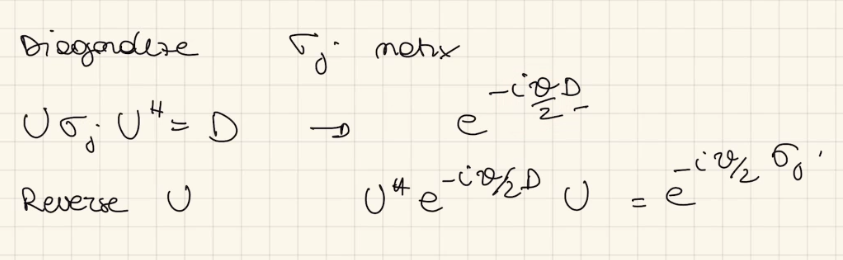
\includegraphics[scale=0.5]{15.png}
\end{center}
$$|00\rangle \rightarrow H\otimes I\rightarrow \frac{|0\rangle+|1\rangle}{\sqrt{2}}|0\rangle\rightarrow\hbox{CNOT}\rightarrow\frac{|00\rangle+|11\rangle}{\sqrt{2}} = |\beta_{00}\rangle$$
$$|01\rangle \rightarrow H\otimes I\rightarrow \frac{|0\rangle+|1\rangle}{\sqrt{2}}|1\rangle\rightarrow\hbox{CNOT}\rightarrow\frac{|01\rangle+|10\rangle}{\sqrt{2}} = |\beta_{01}\rangle$$
$$|10\rangle \rightarrow H\otimes I\rightarrow \frac{|0\rangle-|1\rangle}{\sqrt{2}}|0\rangle\rightarrow\hbox{CNOT}\rightarrow\frac{|00\rangle-|11\rangle}{\sqrt{2}} = |\beta_{10}\rangle$$
$$|11\rangle \rightarrow H\otimes I\rightarrow \frac{|0\rangle-|1\rangle}{\sqrt{2}}|1\rangle\rightarrow\hbox{CNOT}\rightarrow\frac{|01\rangle-|10\rangle}{\sqrt{2}} = |\beta_{11}\rangle$$
\textbf{Every vector is this basis is entangled!}
\paragraph{Sharing a Pair of Entangled Bits}\begin{list}{}{}
	\item The state $|\beta_{00}\rangle$ would have to be created ahead of time, when the qubits are in a lab together and can be made to interact in a way that will give rise to the entanglement between them.
	\item After the state is created, Alice and Bob each take one of the two qubits away with them.
\end{list}
Alternatively, some third party may prepare the entangled state ahead of time and sens one qubit to Alice and the other to Bob.\\\\
If they are careful not to let the qubits interact with the environment or other quantum systems, Alice and Bob's joint state will remain entangled.\\
Note that $|\beta_{00}\rangle$ is a fixed state, there is no need for Alice to have sent any qubit to Bob to prepare this state.
\begin{center}
	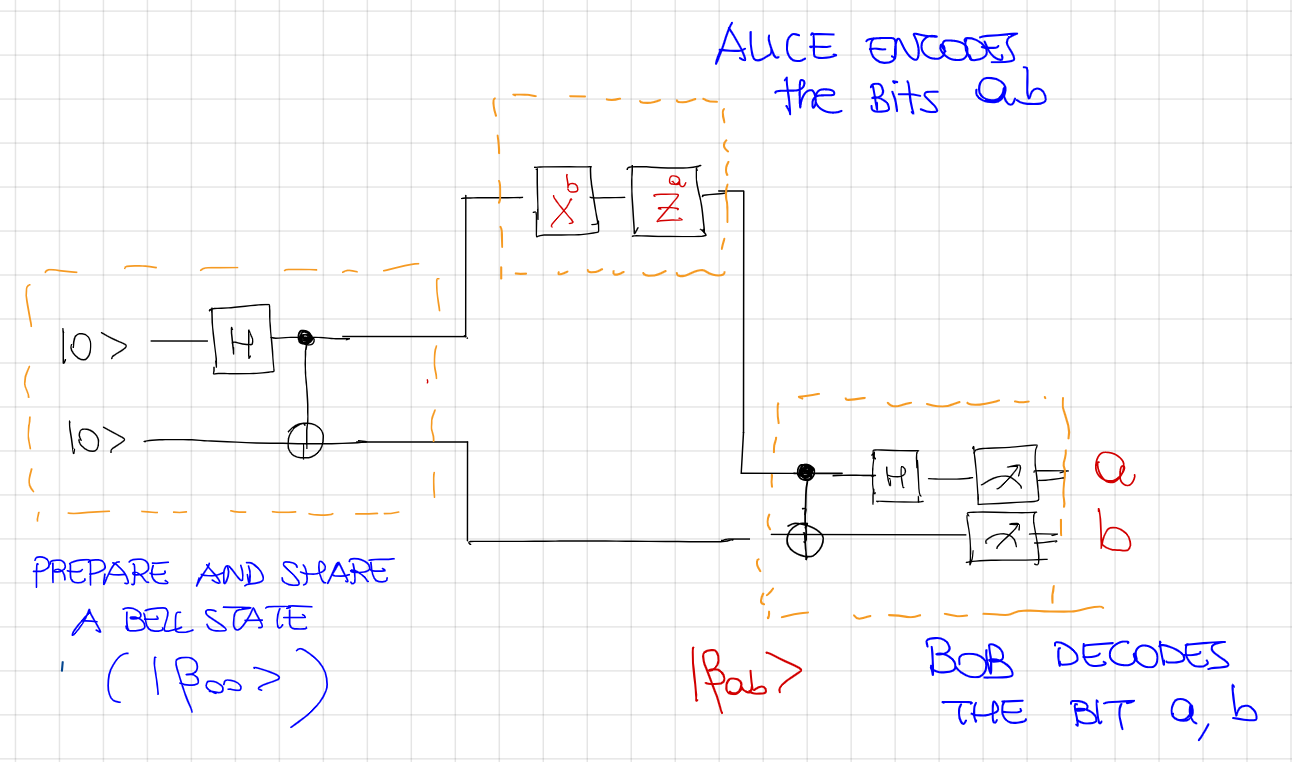
\includegraphics[scale=0.5]{16.png}
\end{center}
\paragraph{Procedure}
\begin{center}
	\begin{tabular}{c c l}
\textbf{To send}&\makecell{\textbf{Alice applies to her}\\\textbf{qubit the gate}}&\textbf{Resulting state}\\
\hline
00&$I$& $|\beta_{00}\rangle \mapsto |\beta_{00}\rangle$ \\
01&$X$& $|\beta_{00}\rangle \mapsto \frac{|10\rangle+|01\rangle}{\sqrt{2}} = |\beta_{01}\rangle$\\
10&$Z$& $|\beta_{00}\rangle \mapsto  \frac{|00\rangle-|11\rangle}{\sqrt{2}} = |\beta_{10}\rangle$\\
11&$ZX$& \makecell{$|\beta_{00}\rangle \mapsto_{X\otimes I}\frac{|10\rangle+|01\rangle}{\sqrt{2}}\mapsto_{Z\otimes I}\frac{-|10\rangle+|01\rangle}{\sqrt{2}}=|\beta_{11}\rangle$}
\end{tabular}
\end{center}
The resulting state is one of the four Bell states, which form an orthonormal basis and can be distinguished by an appropriate quantum measurement. So after applying the appropriate gate, Alice sends her qubit to Bob. Bob is in possession of one of the four Bell states, depending on the classical bits that Alice wished to send him, so he performs a measurement in the Bell basis and determines which bit string Alice sent.\\
The measurement can be implemented by first performing a change of basis, then performing a measurement in the computational basis.\\
The outcome of the Bell measurement reveals to Bob the Bell states he possesses and allows him to determine with certainty the two classical bits.\\
The measurement gives Bob the values $a,b$ corresponding to the Bell state $|\beta_{ab}\rangle$ in his possession.
\paragraph{Example} Alice wants to send $10$, so she applies $Z$ to her qubit
$$|\beta_{00}\rangle = \frac{|00\rangle+|11\rangle}{\sqrt{2}} \mapsto_{Z\otimes I}\frac{|00\rangle-|11\rangle}{\sqrt{2}}$$
and send the qubit to Bob. Bob performs the measurement: applies a CNOT with the first qubit as control and the second as target, then a Hadamard on the first:
$$\frac{|00\rangle-|11\rangle}{\sqrt{2}} \mapsto_{\hbox{CNOT}}\frac{|00\rangle-|10\rangle}{\sqrt{2}}\mapsto_{H\otimes I}\frac{1}{\sqrt{2}}\left(\frac{|0\rangle+|1\rangle}{\sqrt{2}}|0\rangle-\frac{|0\rangle-|1\rangle}{\sqrt{2}}|0\rangle\right)=$$
$$=\frac{1}{2}(\cancel{|00\rangle}+|10\rangle \cancel{-|00\rangle}+|10\rangle) = \frac{1}{2}(2|10\rangle) = |10\rangle$$
Now Bob has the state $|10\rangle$ and know that Alice sent $10$.\\\\
Alice, interacting with only a single qubit, is able to transmit two bits of information to Bob. Two qubits are involved in the protocol, but Alice never need to interact with the second qubit. Classically, the task Alice accomplishes would have been impossible had she only transmitted a single classical bit.\\
Information is physical, and surprising physical theories as Quantum Mechanics may predict surprising information processing abilities.
\paragraph{Communication Channels}
\begin{list}{}{}
	\item \textbf{Quantum Communication Channel} is a communication line (e.g. fiber optic, cable\ldots) which can carry qubits between two remote locations.
	\item \textbf{Communication Channel} is a line that can carry only classical bits (and not qubits).
\end{list}
\paragraph{Quantum Teleportation} Process by which a quantum state is transfered from one location to another, without sending directly the quantum state.\\
Alice has $|\psi\rangle = \alpha|0\rangle+\beta|1\rangle$ and would like to send the quantum state to Bob.\begin{list}{}{}
	\item Alice could physically send the qubit but we rule out this possibility because we want to "teleport".
	\item Alice could tell Bob the amplitude $\alpha$ and $\beta$ for the quantum state $|\psi\rangle$. To do this, she doesn't need to send a quantum state, but she can simply send the complex numbers $\alpha$ and $\beta$ as ordinary classical information e.g. over the internet. Bob could then re-create the state in his lab.\\
	But \textbf{in general Alice doesn't know the identity of her quantum state}.
\end{list}
\textbf{Quantum teleportation works even when the identity of a the state isn't known to Alice or Bob}.
The teleportation instead works like this. The circuit is:
\begin{center}
	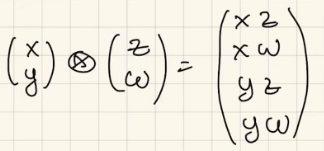
\includegraphics[scale=0.5]{17.png}
\end{center}
Alice has two qubits, Bob just one.
\begin{list}{}{}
	\item \textbf{Step 1}: two qubits are prepared entangled and shared.
	\item \textbf{Step 2}: Alice lets the two qubits interact and measure with a Bell basis measurement, basically by changing the base.
	\item \textbf{Step 3}: Alice measures her two qubits in the computational basis. She has 4 possible equiprobable outcomes.
	\item \textbf{Step 4}: Bob receives the two classical bits from Alice and restores the state $|\psi\rangle$ on his qubit.
\end{list}
No particle have been sent from Alice to Bob, just two classical bits used by Bob to recover the state $|\psi\rangle$. Moving is possible, copying is not possible: $|\psi\rangle$ is not in possession of Alice anymore.\\
Alice measures in the Bell state because: after step one we have $|\psi\rangle|\beta_{00}\rangle$ and you can prove that this is equal to $$|\psi\rangle|\beta_{00}\rangle = \frac{1}{2}(|\beta_{00}\rangle|\psi\rangle + |\beta_{01}\rangle X|\psi\rangle + |\beta_{10}\rangle Z|\psi\rangle + |\beta_{11}\rangle XZ|\psi\rangle)$$
\section{Quantum Algorithms}
The really important question is when quantum computers can outperform classical ones.\\
With a $$f:\{0,1\}\rightarrow\{0,1\}$$ we have 4 functions
\begin{center}
	\begin{tabular}{c | c c c c}
& $f_1$ & $f_2$ & $f_3$ & $f_4$\\
\hline
0 & 0 & 0 & 1 & 1\\
1 & 0 & 1 & 0 & 1
\end{tabular}
\end{center}
With classical algorithms we need two queries to see if a function is balanced or constant. In quantum algorithms we need to query the oracle only once because we can exploit quantum parallelism. Feed the circuit with a superposition of inputs and the oracle returns a superposition of outputs. This is the \textbf{Deutsch algorithm}, and the \textbf{Deutsch problem} is the following: given a black box for computing an unknown function $f:\{0,1\}\rightarrow\{0,1\}$, determine if the function is balanced or constant by making queries to $f$.
\subsection{Classical Computations on Quantum Computers}
We want to compute functions $$f:\{0,1\}^n\rightarrow\{0,1\}$$ We need to have a \textbf{reversible computation}, so unitary gates: can't feed the entire input sequence into a gate. We take any classical logic circuits computing out function, than change each gate into a reversible version. Once we have a computable function with reversible gate than we can translate it into a quantum ambient.\\
To translate a gate into a reversible version we use Toffoli gates, which are reversible versions of the AND. Toffoli gates are C-CNOT. With $C= 0$ is AND, with $C=1$ is a NAND.\\
Toffoli gate and the quantum implementation:
\begin{center}
	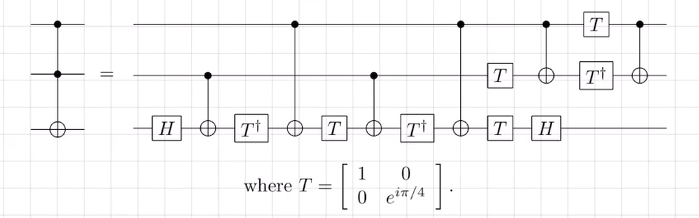
\includegraphics[scale=0.5]{19.png}
\end{center}
Any classical computation can be implemented by a quantum circuit of Toffoli gates.
\paragraph{Quantum Parallelism} An oracle computing a function is a black-box that computes said function. Quantum if used with quantum bits.\\
$U_f$ is implemented, due to reversibility, with input $|x\rangle$ of size $n$ and another qubit $|y\rangle$ used to store the result. The output is $|x\rangle$ and $|y\otimes f(x)\rangle$. It's reversible
$$|x,y\rangle\mapsto_{U_f} |x,y\otimes f(x)\rangle \mapsto_{U_f} |x, (y\otimes f(x))\otimes f(x) \rangle = |x,y\rangle$$
In general $|x\rangle$ is of size $n$, meaning $f:\{0,1\}^n\rightarrow\{0,1\}$. To prepare the $|x\rangle$ (data register) in a superposition we apply the Hadamard gate, and we can generalize this procedure on an arbitrary number of qubits:\begin{center}
	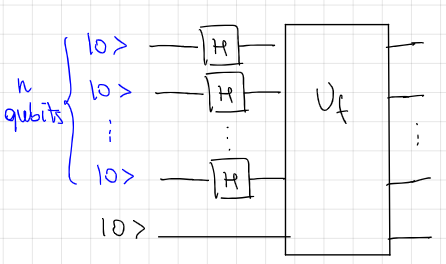
\includegraphics[scale=0.5]{20.png}
\end{center}
So we:\begin{list}{}{}
	\item Prepare the $n+1$ qubit state $|x\rangle^{\otimes n}|y\rangle$
	\item Apply the $H$ gate to the first $n$ qubits, to obtain the equal superposition of all inputs of $f$
	\item Apply the quantum circuit implementing $U_f$
\end{list}
Obtaining the state $\frac{1}{\sqrt{2^n}}\sum_x|x,f(x)\rangle$\\
Quantum parallelism enables all possible values of $f$ to be evaluated simultaneously, even if we evaluate $f$ once. This parallelism is not immediately useful: if we measure the state $\frac{1}{\sqrt{2^n}}\sum_x|x,f(x)\rangle$ we obatin $|x,f(x)\rangle$ for a single value of $x$.\\
To exploit quantum parallelism, we need the ability to extract information about more than one value of $f(x)$ from $\sum_x |x,f(x)\rangle$
\paragraph{Deutsch's Algorithm}
\begin{center}
	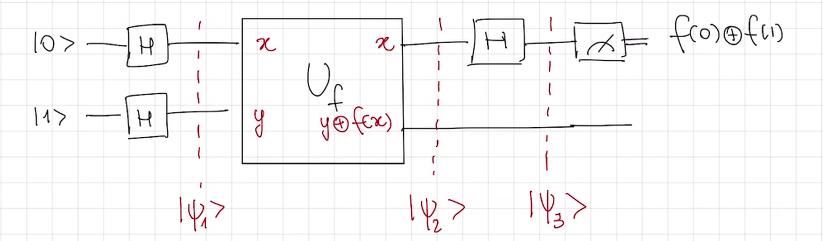
\includegraphics[scale=0.5]{22.png}
\end{center}
$$f(0)\otimes f(1)=\left\{\begin{array}{c l}
0 & f\hbox{ is constant}\\
1 & f\hbox{ is balanced}
\end{array}\right.$$
This circuit solves Deutsch's problem in just one pass. The Hadamard gate on the state $|1\rangle$ is to let the amplitude interfere in order to grasp global properties of the function. The last part measures in the Hadamard basis.
$$|\psi_1\rangle = |+\rangle|-\rangle = \frac{|0\rangle+|1\rangle}{\sqrt{2}}\frac{|0\rangle-|1\rangle}{\sqrt{2}} = \frac{1}{\sqrt{2}}|0\rangle|-\rangle + \frac{1}{\sqrt{2}}|1\rangle|-\rangle$$
Recall that the oracle $U_f$ works like this\begin{list}{}{}
	\item $|x\rangle|-\rangle = |x\rangle\frac{|0\rangle-|1\rangle}{\sqrt{2}} \mapsto_{U_f} |x\rangle\frac{|0\oplus f(x)\rangle - |1\otimes f(x)\rangle}{\sqrt{2}} = |x\rangle\frac{|f(x)\rangle - |\overline{f(x)}\rangle}{\sqrt{2}} = \left\{\begin{array}{l l}
	|x\rangle\frac{|0\rangle-|1\rangle}{\sqrt{2}} = |x\rangle|-\rangle & f(x) = 0\\
	|x\rangle\frac{|1\rangle-|0\rangle}{\sqrt{2}} = -|x\rangle|-\rangle & f(x) = 1
\end{array}	 \right.$\\
	With $\overline{x}$ being the complement of $x$ (if $x=0$ then $\overline{x} = 1$)\\
	So the state doesn't change with $f(x) = 0$ and has a phase factor with $f(x) = 1$. A more compact way is $(-1)^{f(x)}|x\rangle|-\rangle$
\end{list}
So we have $$|\psi_2\rangle = U_f(|+\rangle|-\rangle) = U_f\left(\frac{|0\rangle|-\rangle}{\sqrt{2}}+\frac{|1\rangle|-\rangle}{\sqrt{2}}\right) = \frac{(-1)^{f(0)}|0\rangle|-\rangle + (-1)^{f(1)}|1\rangle|-\rangle}{\sqrt{2}} = \frac{(-1)^{f(0)}|0\rangle + (-1)^{f(1)}|1\rangle}{\sqrt{2}}|-\rangle =$$
$$=\left\{\begin{array}{l l}
\pm\frac{|0\rangle+|1\rangle}{\sqrt{2}}|-\rangle = \pm|+\rangle|-\rangle & f\hbox{ is constant and }f= 0\hbox{ or }1\\
\pm\frac{|0\rangle-|1\rangle}{\sqrt{2}}|-\rangle = \pm|-\rangle|-\rangle & f\hbox{ is balanced and }f(0) = 0, f(1) = 1\hbox{ or viceversa}
\end{array}\right. $$
Then we apply Hadamard on the first qubit
$$|\psi_3\rangle = (H\otimes I)|\psi_2\rangle = \left\{\begin{array}{l l}
\pm (H|+\rangle)|-\rangle& f\hbox{ is constant}\\
\pm (H|-\rangle)|-\rangle& f\hbox{ is balanced}
\end{array}\right. = \left\{\begin{array}{l l}
\pm |0\rangle|-\rangle& f\hbox{ is constant}\\
\pm |1\rangle|-\rangle& f\hbox{ is balanced}
\end{array}\right.$$
With a measure on the computational basis we solve the Deutsch's problem, getting 0 $\Leftrightarrow f$ is constant and $1\Leftrightarrow f$ is balanced.
\paragraph{Deutsch-Jozsa Algorithm} Generalization of the Deutsch's problem
$$f:\{0,1\}^n\rightarrow\{0,1\}$$
As input we have a black box for computing an unknown function $f:\{0,1\}^n\rightarrow\{0,1\}$ either constant or balanced.\\
The problem is to determine whether $f$ is constant or balanced.\\\\
Classical (exact) solution, in the best case we query twice getting two different answers, then $f$ is balanced for sure. The worst case is $2^{n-1}$ queries with the same result, so $2^{n-1}+1$ queries: if the last value is different then is balanced, otherwise is constant. So classically we need an exponential number of queries. With quantum circuits we do just one query.
\begin{center}
	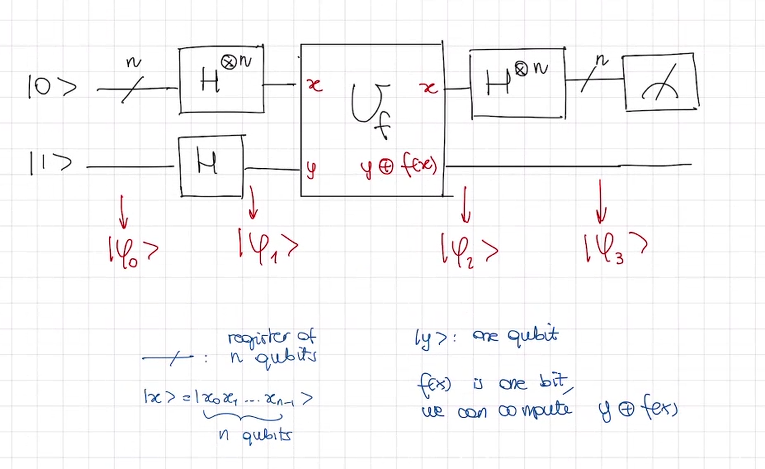
\includegraphics[scale=0.5]{23.png}
\end{center}
Very similar, just with a $n$ qubits on state $|0\rangle$ in the query register and 1 qubit in state $|1\rangle$ in the answer register.
$$|\psi_0\rangle = |0\ldots 0\rangle|1\rangle = |0\rangle^{\otimes n}|1\rangle$$
$$|\psi_1\rangle = \sum_{x\in\{0,1\}^n}\frac{|x\rangle}{\sqrt{2}}|-\rangle$$
Query register: uniform superposition of all values.\\
Answer register: uniform superposition of state $|0\rangle$ and $|1\rangle$.
$$|\psi_2\rangle = \frac{1}{\sqrt{2^n}}U_f\left(\sum_{x\in\{0,1\}^n}|x\rangle|-\rangle\right) = \frac{1}{\sqrt{2^n}} \sum_{x\in\{0,1\}^n} U_f(|x\rangle|-\rangle) = \frac{1}{\sqrt{2^n}} \sum_{x\in\{0,1\}^n} (-1)^{f(x)}|x\rangle|-\rangle$$
Let's see on a single qubit
$$H|x_i\rangle = \frac{|0\rangle+(-1)^{x_i}|1\rangle}{\sqrt{2}} = \frac{1}{\sqrt{2}} \sum_{z_i\in\{0,1\}} (-1)^{x_i}|z_1\rangle=\left\{\begin{array}{l l}
\frac{1}{\sqrt{2}}\frac{|0\rangle+|1\rangle}{\sqrt{2}} & x_i = 0\\
\frac{1}{\sqrt{2}}\frac{|0\rangle-|1\rangle}{\sqrt{2}} & x_i = 1\\
\end{array}\right.$$
So we have
$$H^{\otimes n}|x\rangle = (H|x_0\rangle)\ldots(H|x_{n-1}\rangle) = \frac{1}{\sqrt{2}}\left(\sum_{z_0=0}^1(-1)^{x_0z_0}|z_0\rangle\right)\ldots\left(\sum_{z_{n-1}=0}^1(-1)^{x_{n-1}z_{n-1}}|z_{n-1}\rangle\right)=$$
$$=\frac{1}{\sqrt{2^n}} \sum_{z_0=0}^1\ldots\sum_{z_{n-1}=0}^1 (-1)^{x_0z_0+\ldots+x_{n-1}z_{n-1}}|z_0\rangle\ldots|z_{n-1}\rangle = \frac{1}{\sqrt{2^n}}\sum_{z\in\{0,1\}^n} (-1)^{x\cdot z}|z\rangle$$
So
$$|\psi_3\rangle = H^{\otimes n}\left(\frac{1}{\sqrt{2^n}}\sum_x(-1)^{f(x)}|x\rangle \right)|-\rangle = \frac{1}{\sqrt{2^n}}\left(\sum_x (-1)^{f(x)}H^{\otimes n}|x\rangle\right)|-\rangle =$$ $$= \frac{1}{\sqrt{2^n}}\left( \sum_x (-1)^{f(x)}\frac{1}{\sqrt{2^n}}\sum_{z\in\{0,1\}^n}(-1)^{x\cdot z}|z\rangle\right)|-\rangle = \frac{1}{2^n}\sum_{z\in\{0,1\}^n}\left(\sum_{x\in\{0,1\}^n}(-1)^{f(x)+x\cdot z}|z\rangle\right)|-\rangle$$
Let's consider the amplitude of the state $|z\rangle = |0\ldots 0\rangle$
$$\frac{1}{2^n}\sum_{x\in\{0,1\}^n}(-1)^{f(x)+0} = \frac{1}{2^n}\sum_{x\in\{0,1\}^n}(-1)^{f(x)}=\left\{\begin{array}{l l}
-1&f\hbox{ is constant and }=0\\
+1&f\hbox{ is constant and }=1\\
0&f\hbox{ is balanced}\\
\end{array}\right.$$
So if $f$ is constant, the amplitude of $|0\ldots0\rangle$ is $\pm 1$ (all other amplitudes are 0 since $|\psi_3\rangle$ is a unit vector), and a measurement in the computational basis is certain to return all zeroes (the binary string 0\ldots 0).\\
If $f$ is balanced, positive and negative contributes cancel each other and the overall amplitude is 0, the measurement is certain not to return all zeroes.
\paragraph{Probability Error} $$2\left(\frac{1}{2}\right)^k = \frac{1}{2^{k-1}}$$
\paragraph{Simon's Algorithm} $$f:\{0,1\}^n\rightarrow\{0,1\}^n$$
Is $f$ one-to-one (bijection) or two-to-one function?
\subsection{Quantum Fourier Transform}
Building block for many important algorithms: QPE, QAA, Shor's, QS\ldots
\paragraph{Discrete Fourier Transform} DFT, essentially multiplying a unitary matrix by a vector. With Fast Fourier Transform we do it in $O(N\log N)$ with $N = 2^n$.\\
We have $x_0,\ldots,x_{N-1}$ and $y_0,\ldots,y_{N-1}$ 
Primitive root of unity $\omega_N = e^{\frac{2\pi i}{N}}$
$$y_N = \frac{1}{\sqrt{N}} = \sum_{j=0}^{N-1} e^{\frac{2\pi ijk}{N}}x_j= \sum_{j=0}^{N-1} \omega_N^{jk}x_j$$
So we have $$y = F_N x$$ with $F_N$ unitary matrix, given by the $k$ indexes. $k=0$ we have all ones in the first row.
$$F_n = \frac{1}{\sqrt{N}}\left[\begin{array}{c c c c}
1 & \ldots & \ldots & 1\\
1 & w_N & \ldots & \omega_N^{N-1}\\
\vdots\\
1
\end{array}\right]$$
$$w_N^{kj}\hbox{ in positions }k,j=0,\ldots,N-1$$
The conjugation of $w_N^{jk}$ is $\cos \pm i\sin$ changing the sign.
$$F_N\cdot F_N^H = \frac{1}{N}\left[\begin{array}{c}
w_{kj}
\end{array}\right]\left[\begin{array}{c}
w_{sp}^{-1}
\end{array}\right] = $$
$F_N$ needs to be unitary so this multiplication must be $I$, so $(F_N\cdot F_N^H)_{st}=\left\{\begin{array}{l l}
0&s\neq t\\
1&s = t
\end{array}\right.$\\
It's provable that $\sum_{j=0}^{N-1}\omega_N^{kj}=\left\{\begin{array}{l l}
N&k= 0\hbox{ mod }N\\
0&k\neq 0\hbox{ mod }N
\end{array}\right.$\\
So essentially we have $$(F_NF_N^H)_{st} = \frac{1}{N}\sum_{j=0}\omega_N^{js}\omega_N^{-jt}= \frac{1}{N}\sum_{j=0}^{N-1}\omega_N^{j(s-t)}$$
So it's unitary %TODO proof
\subparagraph{Example} $n=1, N=2$ $$F_2=\frac{1}{\sqrt{2}}\left[\begin{array}{c c}
1&1\\1&-1
\end{array}\right] = H$$
$$\omega_2 = \cos\pi + i\sin\pi$$
\paragraph{Quantum Fourier Transform} We're in the quantum world, so we're working with quantum states. When we measure we collapse from a state, losing the superposition.\\
$|y\rangle = H^{\otimes n}|x\rangle$ is already a quantum Fourier transform, over a group $Z_2\otimes Z_2\otimes\ldots\otimes Z_2$, binary.\\
Thanks to Coppersmith in 1994, we pass from $O(N\log N) = O(2^n n)$ of the fast (classical) Fourier transform to the $O(n^2)$ of the quantum one, so from exponential to polynomial: an exponential speedup. But they don't compute the same quantities.\\\\
We define QFT on an orthonormal basis $$|0\rangle,|1\rangle\ldots|N-1\rangle$$
$$|\tilde{j}\rangle = QFT(|j\rangle)$$
More in general, with $$x=\sum_{j=0}^{N-1} x_j|j\rangle$$ $$|\tilde{x}\rangle = QFT(|x\rangle)$$
To define, we start from the classical definition applying to each element of the basis
$$|\tilde{j}\rangle = QFT(|j\rangle) = \frac{1}{\sqrt{N}}\sum_{k=0}^{N-1} e^{\frac{2\pi ijk}{N}}|k\rangle$$
So QFT transforms from the canonical $Z$ basis (computational basis) to the Fourier basis.
\subparagraph{Example} $n=1$, 1-qubit
\begin{center}
	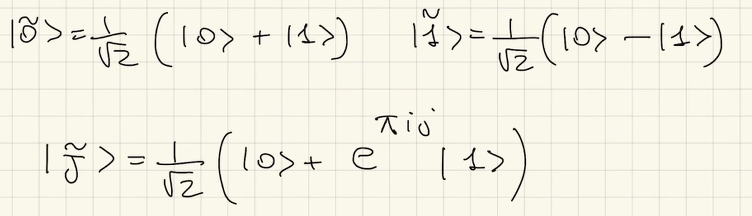
\includegraphics[scale=0.5]{24.png} %TODO rewrite, guarda lezione
\end{center}
\subparagraph{$N$-qubits System}\begin{list}{}{}
	\item Write QFT formally
	\item Use some rewriting to get the circuit
\end{list}
With 1-qubit, $\{|0\rangle,|1\rangle\}$. With 2-qubit $\{|0\rangle,|1\rangle,|2\rangle,|3\rangle\}$ which is a short-hand writing of $\{|00\rangle,|01\rangle,|10\rangle,|11\rangle\}$.\\
With $N$-qubits we have the basis $\{|0\rangle,|1\rangle,\ldots,|N-1\rangle\}$ keeping in mind that it's a short-hand writing, $2^n$ basis states so $2^n$ configuration of bits. E.g. $|4\rangle = |100\rangle$\\\\
$n=3$ $$|\tilde{j}\rangle = \frac{1}{\sqrt{8}}\sum_{k=0}^{2^3-1}e^{\frac{1\pi ijk}{8}}|k\rangle$$
Remembering that
$$|k\rangle=|k_1k_2k_3\rangle$$
So the sum must be interpreted as $$\sum_k = \sum_{k_1=0}^1\sum_{k_2=0}^1\sum_{k_3=0}^1$$
In the general case
$$|\tilde{j}\rangle = \frac{1}{\sqrt{N}}\sum_{k=0}^{N-1}e^{\frac{2\pi ijk}{2^n}}|k\rangle =$$
with $k=k_1k_2\ldots k_n$ which are digits of the binary representation, so can be rewritten in decimal representation as $k = \sum_{s=1}^n k_s2^{n-s}$
$$= \frac{1}{\sqrt{N}}\sum_{k=0}^{N-1}e^{2\pi ij\sum_{s=1}^n k_s2^{-s}}|k_1\ldots k_n\rangle =$$
$$=\frac{1}{\sqrt{N}}\sum_{k=0}^{N-1}\prod_{s=1}^n e^{\frac{2\pi ij k_s}{2^s}}|k_1\ldots k_n\rangle =$$
If you isolate the first qubit you get a tensor product because of the $\prod$, and the $sum_k$ decomposes into the sums $sum_{k_1}\sum_{k_2}\ldots$
$$=\frac{1}{\sqrt{N}}\left(|0\rangle+e^{\frac{2\pi ij}{2^1}}|1\rangle \right)\otimes\left(|0\rangle+e^{\frac{2\pi ij}{2^2}}|1\rangle \right)\otimes \ldots\otimes \left(|0\rangle+e^{\frac{2\pi ij}{2^n}}|1\rangle \right)$$
Each qubit has been transformed into something very similar to an Hadamard gate, except for the exponent of $e$.\\
So we went from $$|j\rangle = |j_1\ldots j_n\rangle = |j_1\rangle\otimes\ldots\otimes|j_n\rangle$$ to $$|\tilde{j}\rangle=\frac{1}{\sqrt{N}}\left(|0\rangle + e^{\frac{2\pi ij}{2^1}}|1\rangle\right)\otimes\ldots\otimes\left(|0\rangle + e^{\frac{2\pi ij}{2^n}}|1\rangle\right)$$
with a 1 to 1 correspondence between bits.
$$|j_s\rangle\mapsto|\tilde{j}_s\rangle=\left(|0\rangle +e^{\frac{2\pi ij}{2^s}}|1\rangle\right)$$
Each gets a bit of information from each configuration, with $s$ affecting the relative phase.
\begin{list}{}{}
	\item $\frac{1}{\sqrt{N}} e^{\frac{2\pi i j}{2}} \rightarrow |10\ldots0\rangle$
	\item $\frac{1}{\sqrt{N}} e^{\frac{2\pi i j}{2^n}} \rightarrow |0\ldots01\rangle$
	\item $\frac{1}{\sqrt{N}} e^{\frac{2\pi i j}{2^s}} \rightarrow |0\ldots010\ldots0\rangle$
	\item $\frac{1}{\sqrt{N}} \left(e^{\frac{2\pi i j}{2}} +\ldots+e^{\frac{2\pi i j}{2^n}}\right) = \frac{1}{\sqrt{N}}e^{2\pi i(\frac{j}{2}+\ldots +\frac{j}{2^n})} \rightarrow |1\ldots1\rangle$
\end{list}
So the the phase applied is qubit dependent
\subparagraph{Example} $n=3, |j\rangle=|101\rangle$
$$|\tilde{5}\rangle = \frac{1}{N}\left(|0\rangle + e^{2\pi i\frac{5}{2}}|1\rangle\right)\otimes\left(|0\rangle + e^{2\pi i\frac{5}{4}}|1\rangle\right)\otimes\left(|0\rangle + e^{2\pi i\frac{5}{8}}|1\rangle\right)$$
\paragraph{Building Blocks for the Circuit}\begin{list}{}{}
	\item $H|j_s\rangle\mapsto\frac{1}{\sqrt{2}}\left(|0\rangle+e^{\frac{2\pi i}{2}j_s}|1\rangle\right)$
	\item Something that depends on the index and does the right rotation: the $U_s$ rotation gate depending on $s$.\\
	$U_s|j_t\rangle\mapsto e^{\frac{2\pi i }{2^s}j_t}|j_t\rangle$\\
	Just applies a phase.
	\item 
\end{list}
\paragraph{The Circuit}
\begin{center}
	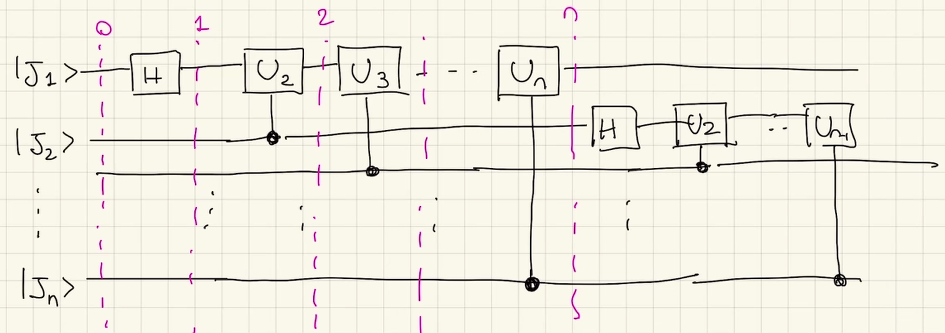
\includegraphics[scale=0.5]{25.png}
\end{center}
\begin{enumerate}
	\item $|j_1\ldots j_n\rangle$
	\item $H|j_1\rangle = \frac{1}{\sqrt{2}}\left(|0\rangle e^{\frac{2\pi i}{2}j_1}|1\rangle\right)\otimes |j_2\ldots j_n\rangle$
	\item Apply the gate only when $j_2$ is 1 (the black dot means that), but that's how $U$ works, it has a 0 on the $|0\rangle$\\
	$\frac{1}{\sqrt{2}}\left(|0\rangle+e^{\frac{2\pi i}{2}j_1}e^{\frac{2\pi i}{2^2}j_2}|1\rangle\right)\otimes|j_2\ldots j_n\rangle$
	\item $\frac{1}{\sqrt{2}}\left(|0\rangle+e^{\frac{2\pi i}{2}j_1}e^{\frac{2\pi i}{2^2}j_2}e^{\frac{2\pi i}{2^3}j_1}|1\rangle\right)\otimes|j_2\ldots j_n\rangle$
	\item[] \ldots
	\item[$n$.] $\frac{1}{\sqrt{2}}\left(|0\rangle+e^{2\pi i(\frac{j_1}{2}+\frac{j_2}{2^2}+\ldots+\frac{j_n}{2^n})}|1\rangle\right)\otimes|j_2\ldots j_n\rangle=$\\
	And given that 
	$j = \sum_{s=1}^nj_s 2^{n-s} = j_1 2^n+j_s^{n-1}+\ldots +j_n 2^0$ so we have
	$\frac{j_1}{2}+\frac{j_2}{2^2}+\ldots+\frac{j_n}{2^n} = \frac{1}{2^n}(j_1 2^n+j_s^{n-1}+\ldots +j_n 2^0)$ we have that\\
	$=\frac{1}{\sqrt{2}}\left(|0\rangle + e^{\frac{2\pi ij}{2^n}}|1\rangle\right)\otimes |j_2\ldots j_n\rangle$\\
	But we end up with the $n$th configuration on the first qubit!
\end{enumerate}
So we implements QFT in the reverse order, applying for example swap gates at the beginning or changing the configuration of the qubits at the end.
\end{document}
